\documentclass[a4paper]{article}
\usepackage[utf8]{inputenc}
\usepackage[dvipsnames]{xcolor}
\usepackage[hidelinks]{hyperref}
\usepackage{graphicx, amssymb, amsfonts, color, todonotes, diagbox, colortbl, pdfpages, listings, amsmath, caption, subcaption, xspace, xcolor, pifont, fullpage, algorithm, algpseudocode}
\algnewcommand\algorithmicforeach{\textbf{for each}}
\algdef{S}[FOR]{ForEach}[1]{\algorithmicforeach\ #1\ \algorithmicdo}
\setlength{\parskip}{0.2 cm}
\newtheorem{definition}{Definition}
\newtheorem{theorem}{Theorem}
%~ \usepackage{amsmath}
% Commands
\newcommand{\Node}[1]{\ensuremath{\mathrm{Node}_{#1}}\xspace}
\newcommand{\flow}[1]{\ensuremath{\mathit{flow}_{#1}}\xspace}
\newcommand{\inputs}{\ensuremath{\mathcal{F}}\xspace}
\newcommand{\memory}{\ensuremath{\mathcal{M}}\xspace}
\newcommand{\memorymap}{\ensuremath{\mathcal{M}_{map}}\xspace}
\newcommand{\duration}{\mathit{Duration}\xspace}
\newcommand{\bandwidth}{\mathit{BW}\xspace}
\newcommand{\core}{\mathit{Cores}\xspace}
\newcommand{\submissiontime}{\mathit{Subtime}\xspace}
\newcommand{\walltime}{\mathit{Walltime}\xspace}
\newcommand{\completiontime}{\mathit{Completiontime}\xspace}
\newcommand{\start}{\mathit{Starttime}\xspace}
\newcommand{\fileset}{\ensuremath{\mathbb{F}}\xspace}
\newcommand{\jobset}{\ensuremath{\mathbb{J}}\xspace}
\newcommand{\evict}{\ensuremath{\mathcal{V}}\xspace}
\newcommand{\nbloads}{\ensuremath{\mathit{\mathit{Loads}}}\xspace}
\newcommand{\live}{\ensuremath{L}\xspace}
\renewcommand{\algorithmicrequire}{\textbf{Input:}}
\renewcommand{\algorithmicensure}{\textbf{Output:}}

\title{Data Aware Batch Scheduling}
\author{Maxime GONTHIER - Carl NETTELBLAD - Elisabeth LARSSON \\ Samuel THIBAULT - Loris MARCHAL}
\usepackage[backend=bibtex]{biblatex}
\bibliography{ref}

\begin{document}

\maketitle
\tableofcontents
\listoffigures
\newpage

\todo[inline]{Maxime: You can add highlighted comments this way: "\textbackslash todo[inline]\{Text\}".}
\todo{Maxime: Or with: "\textbackslash todo\\\{Text\}".}

\section{Motivation}

When using a HPC cluster, users may submits tens to hundreds jobs using the same multi-GB input file.
Users tend to submit each such run as a separate batch job.
The job will read inputs directly from a shared file system, which can be disastrous if the number of I/O are important.
We can thus ask ourselves, \textbf{how can we minimize the amount of transfers between the shared file system and the nodes ?}

Users can manually group together input files into a single job to reduce the effects from I/O reads.
Ideally, we would like to let the user submit jobs the way they want and schedule efficiently jobs on nodes.
The workers have a way to store files (with a limit on the memory size).
%~ as well as a cache page which contains the files/data recently used.
Thus, a way to minimize data transfers is to create a scheduler that \textbf{take into consideration data locality and schedule on the same node jobs sharing inputs}.

Our scheduler would be used to \textbf{distribute the load between the workers but also to have a vision of what the memory of each worker contains in order to re-use as much as possible a file already loaded on a worker's local memory}.

Clusters already use the efficient SLURM scheduler in order to distribute jobs.
\textbf{Thus our goal is to replace SLURM's default scheduler.}

\section{Related Work}

\subsection{The current state of SLURM}
SLURM~\cite{SLURM} is a cluster resource management system, flexible, fault-tolerant and highly scalable.
%~ Schedulers are part of the standard configuration.
First, jobs are scheduled in the FCFS order. 
On top of that, the Backfill algorithm is very widely used~\cite{New_Backfill}.
Backfill is, most often, based on the First Come - First Served principle as well. While the scheduler is running, jobs in the queue are sorted by priority and queueing time~\cite{New_Backfill}.
Then, Backfill will start immediatly all jobs that can be started and completed without delaying the planned schedule.
%~ If there are not enough nodes to start a job, Backfill takes the next job from the queue and sets it for execution if there are enough nodes for this job and it does not delay other jobs.
This algorithm allows to increase the density of supercomputer ressources' use by 20\% as well as reducing the average waiting time
for execution~\cite{Maui_Scheduler}.
There are two types of backfills. Coservative and EASY. Conservative backfill jobs that do not delay all other jobs. EASY backfill jobs that do not delay only the first scheduled job.
EASY backfill is known to be efficient and able to prevent starvation~\cite{easybf}.
\textbf{Thus our main competitor will be the EASY-Backfill algorithm.}

\subsection{Other ways to improve SLURM and other batch systems}
To deal with communication-intensive jobs on SLURM, a solution is to minimize network contention by allocating nodes on the least
contended switches~\cite{minimize_network_contention}. In our case we have
jobs with one large file transfers that must be done before the computation start, which is different.
Furthermore, we are scheduling further down the topology (i.e nodes and not switches).

In "Explicit Control in a Batch-Aware Distributed File System"~\cite{Explicit_Control_in_a_Batch-Aware_Distributed_File_System},
we are presented with "Batch-Aware Distributed File System", a system designed to orchestrate large, 
I/O-intensive batch workloads on remote computing clusters.
It adds "storage servers" that export access to the disk. And a scheduler that
manage jobs. 
Like us, they use detailed knowledge of workload characteristics.
However, the main idea is not data reuse but to
facilitates the execution of I/O intensive batch
jobs by selecting appropriate storage policies
in regards to I/O scoping (creating a custom environment for each job
for data that will be used a lot by the job, thus not accessing the main disk too
much) and space allocation.


\subsection{Other papers about memory-aware scheduling}
Memory-aware scheduling on clusters have been studied in the past.
 
"Algorithmic Modifications to the
Jacobi-Davidson Parallel Eigensolver to Dynamically Balance External CPU and Memory Load"~\cite{loadbalance_and_trashing} tackle both load balancing and memory constraint. For the load balancing, they 
estimate the time needed by the fastest processor to perform the required $m$ jobs. Thus they can equilibrate the load
with this information. In our study we could use a similar strategy by estimating the 
processing time of a job, the length of a file transfer, and the amount of file transfers needed.
To deal with memory constraint the strategy applied in the paper is to check if 
nodes are thrashing data. If yes, it will recede execution of jobs on this node.
The main differences are that they are using dynamic jobs. Also, we would like to 
manage eviction and optimize data reuse during the scheduling phase, instead of
receding execution on nodes.

Some researchers~\cite{Nikolopoulos2003AdaptiveSU}
are focusing on a better utilization of idling memory together with 
thrashing limitation. Our focus will be to control data loads and eviction so the
processing order will naturally limits thrashing.

\subsection{HDFS, a popular distributed file system}
HDFS~\cite{hdfs} or Hadoop Distributed File System is a distributed file system that incorporate memory-aware scheduling.
HDFS is suitable for applications that have large data sets. 
"Moving Computation is Cheaper than Moving Data" is an important idea for HDFS.
It will migrate a computation closer to where the data is located rather than moving the data to where
the application is running.
Here are our main differences with HDFS. Firstly, HDFS is made for commodity hardware, prone
to more errors and breakdown, so to minimize the risk of failure, data are redundant on the nodes.
In our use case, the scheduler will run on professional clusters and the main point is to load as 
little data as possible. Secondly, HDFS is mainly a storage system, with metadata as transactions historic or
block location. Those concept are not relevant in our use case. Thirdly, the scheduling 
can have issues. A paper describe in detail some problems from MapReduce~\cite{issue_with_hdfs}, the
programming language used in HFDS: the static configuration of the memory allocation, the one-task assigned buffers, the
lake of concurrent task running strategy and the I/O negative impact in memory during the shuffling phase.
To resolve these issues, Mammoth~\cite{Mammoth} was created. It optimize memory usage on a node depending on the hardware configuration.
Our approach is different because we are not dealing with MapReduce or memory allocation.
Our approach is upstream. We can only allocate jobs to nodes. Moreover, we would like to maintain
equity among users  while optimizing I/O.
In addition, HDFS is particularly efficient when the input data used are identical over time.
In our case, one user will submit a lot of different jobs using the same data, but between users,
the inputs are not the same. So HDFS would be less efficient.


\section{Problem Modeling}

\subsection{Framework}

We consider the problem of scheduling a set of independent jobs $\jobset$ on $K$ nodes,
denoted by $\Node{1},\ldots, \Node{K}$.

\subsubsection{Nodes}
Each node is equipped with $N$ cores noted: $\Node{1}(C_1, C_2, ..., C_{N})$.
Let's note $\mathbb{M} = M_1, M_2, ..., M_l$ the set of available memory sizes, with $M_1 < M_2 < ... < M_l$.
Each node has a limited memory $\memory(\Node{i})$ such that $\memory(\Node{i}) \in \mathbb{M}$.

\subsubsection{Input files}
We denote by $\fileset = F_1, F_2, ..., F_n$ the set of input files.
Each file has a size in GB noted $\memory(F_i)$. 
The size of a file is proportional to the number of cores requested by the job using the file.
This size is thus a multiple of $\frac{M_i}{N}$, $M_i \in \mathbb{M}$.

\subsubsection{Jobs}
We denote by $\jobset$ the set of jobs.

We denote by $\inputs(J_i)$ the input file required by job $J_i$. $\inputs(J_i)$ can be empty.
Each job request a certain number of cores $\core(J_i)$. 
For each $j$, $\memory(\inputs(J_j)) = \frac{M_i}{N} \times \core(J_j)$, $M_i \in \mathbb{M}$.

Each job has a submission time $\submissiontime(J_i)$ and a walltime $\walltime(J_i)$.
A job can request between 1 and $N$ cores.

With this model there cannot be any situation in which the memory is fully used
but the cores are not. Because these two values are related to each other. 
However we can have situation where the memory is not fully used but the cores are,
for example if a $N$ cores job using a file $i$ such that $\memory(F_i) = M_1$ is schedule a node with a $M_2$ memory.

Initially, all input files are stored in the main shared file system.
During the processing of a job $J_i$ on $\Node{k}$,
$\inputs(J_i)$ must be in the memory of $\Node{k}$. 
We do not consider the data output of jobs.
Each of the $m$ jobs must be processed on some of the $K$ nodes. 
We consider that all jobs are single nodes.

The file sharing system initially contains all of $\fileset$.
Each node is connected to the file sharing system with a limited bandwidth.
Each node has the same bandwidth noted $\bandwidth$.
The bounded bandwidth as well as the sizes of the files are the reasons why
we aim at restricting the amount of data movement.

The memory of a node is used only by physical writing of files and denoted by $\memory(\Node{i})$.
A file can be shared by two jobs $J_i$ and $J_j$ only in the following situations:
\begin{enumerate}
	\item $J_i$ and $J_j$ are computed in parallel on the same node.
	\item $J_i$ and $J_j$ are computed on the same node consecutively.
\end{enumerate}
Otherwise we consider that memory operations will cause the files to be evicted.

We now define more formally the allocation of the jobs to the node and
their schedule.
We denote by $\sigma(k,i)$ the $i^\text{th}$ job
processed on $\Node{k}$ and by $\evict(k,i)$ the set of file to
be evicted from the memory of $\Node{k}$ before the processing
of this $i^\text{th}$ job ($\evict(k,i)$ can be empty if there is enough space to fit the new files).

On $\Node{k}$, the schedule is made of a
succession of $\mathit{nb}_k$ (the number of jobs allocated) steps, each step being composed of the
following stages (in this order):
\begin{enumerate}
\item The input files in $\inputs(J_{\sigma(k,i)})$ that are not yet in memory are loaded in the memory of $\Node{k}$;
\item Job $J_{\sigma(k,i)}$ is processed on $\Node{k}$ during at most $\walltime(J_i)$.
\end{enumerate}
It is important to note that the file transfers are done before the computation and can not be overlapped.

We are in a Non-Preemptive case, so we cannot stop a job and resume it later.

\subsection{Formalization of the objective}
\textbf{Objective: Minimize the \flow{} stretch}
		We define the \flow{J_i} of a job as:
		$$
			\flow{J_i} = \completiontime(J_i) - \submissiontime(J_i)
		$$
		The flow stretch is the ratio between the flow of a job and the time it would have taken to complete the job on an empty cluster.
		$$
			\textbf{Obj.}: \quad \mathit{minimize}~\frac{\sum_{i=0}^{|\jobset|}\frac{\flow{J_i}}{\duration(J_i) + \frac{\memory(\inputs(J_i))}{\bandwidth}}}{|\jobset|}
		$$
A secondary objective is to minimize the amount of file load.

\section{Other measurements}

Each job has a start time $\start(J_i)$, the actual time at which the job was executed.
We also want to make sure that the maximum queue time of a job is not significantly higher that other methods's maximum queue time with our schedulers.
$$
	Queue_{J_i} = \start(J_i) - \submissiontime(J_i)
$$
$$
	Maximum\_queue\_time = max(Queue_{J_1}, Queue_{J_2}, ..., Queue_{J_m})
$$

\section{Experimental settings}

In our case we will be using the Rackham cluster. The reason is to both have
real cluster information as well as real history of jobs submitted by users.
From the rackham cluster we extract the following parameters:
\begin{itemize}
	\item There are $K = 486$ nodes.
	\item There are $l = 3$ different nodes sizes: $\mathbb{M} = 128, 256, 1024$.
	\item For $i \in [1,450]$, $\memory(\Node{i}) = 128$.
	\item For $i \in [451,482]$, $\memory(\Node{i}) = 256$.
	\item For $i \in [483,486]$, $\memory(\Node{i}) = 1024$.
	\item Each node has $N = 20$ cores.
	\item The bandwidth of each node is $\bandwidth = 0.1 GB/s$.
\end{itemize}

We can extract from Rackham's history, the set of jobs that ended each day, with information on the submission time, walltime, cores asked
and real execution time of each job.
A job is rarely running for more than a week.

Let's say we want to evaluate jobs submitted on day 1.
In order to do this we first look at all the jobs that ended between day 0 and 8.
This should be enough to cover the ending times of most of the jobs submitted on day 1 because most jobs do not last for more than 7 days.
We sort these jobs by submission time. 
The jobs can fall in two different cases:
\begin{itemize}
	\item From the workload history, it started before day 0. So we start it on the node and at the time written in the workload history
	\item From the workload history, it started after day 0. So, this job is not schedule beforehand, it's just in the queue of available jobs like all other jobs.
\end{itemize}
This gives us a fixed representation of what the cluster would have looked like on the dawn of day 0. The main benefit is that this starting point is the same for all schedulers.
Jobs from day 0 are ignored to limit the effect of bulk of jobs we could get with jobs submitted before day 0.
For the same reasons, jobs submitted after day 1 are scheduled but not evaluated.
Jobs from day 0 to 8 are all scheduled but only jobs from day 1 are evaluated.

In order to evaluate our schedulers focused on file re-use, we need to incorparate input files for each jobs. This information is not know from the workload's history, we must create it as follow:
\begin{itemize}
	\item Each job has an input file.
	\item A file is shared between two jobs if they are submitted by the same user in a $800$ seconds timeframe and are using the same number of cores.
\end{itemize}

From the workloads history, we observed that only a small portion of jobs use input files
requiring 256 or 1024GB nodes. Thus for our experiments we will consider that when a file is created, it has 
a 5\% chance to require a 1024 node and a 10\% to require a 256 GB node.

%~ \section{The use of simulation}

%~ The use of simulation is motivated both by the fidelity of simulated results as well as energy savings. 
%~ We will be using Batsim, a precise and realistic~\cite{Batsim} resource and job management system (RJMS) simulator.
%~ Batsim JSON-formatted workloads are extensible and allow easy workload generation. 
%~ Moreover, Batsim provides clear information about scheduling metrics and job placement.
%~ We will add a scheduler using Batsched~\footnote{\url{https://gitlab.inria.fr/batsim/batsched}}.

%~ \paragraph{Data mining for an accurate simulation}
%~ We are matching Uppsala's University cluster Rackham:
%~ \begin{itemize}
	%~ \item	Bandwidth of each node: Let's stick with 100 MB/s as the BW for writing
	%~ \item	Size of input files: 800 to 0GB
	%~ \item	Duration of jobs: from real data
	%~ \item	Total number of jobs: from real data
	%~ \item	Number of available nodes: 486 max. We can test with different number ranging from 20 to 486
	%~ \item	Size of node's memory: 4 of 1TB, 32 of 256GB and the rest has 128GB : A file larger won't be accepted. You need to use the 1TB node if your file is too large.
%~ \end{itemize}

%~ \paragraph{How to simulate data transfers ?}
%~ We can add dynamic job of duration the time it would take to transfer the file on the node in order
%~ to simulate file loads.

\section{Algorithms}

When we need to choose a node for job $J_i$ we know the following informations:
\begin{itemize}
	\item $\submissiontime(J_i)$
	\item $\walltime(J_i)$
	\item $\inputs(J_i)$
	\item Size of files for the job: $\memory(\inputs(J_i))$
	\item For each $i$, $\inputs(\Node{i})$
	\item Size of files already on memory of the node: For each $i$, $\memory(\inputs(\Node{i}))$
	\item Bandwidth: $\bandwidth$
\end{itemize}

\subsection{Maximum use single file}
\paragraph{Intuition}
Find the file shared the most among available jobs.
Schedule all jobs using this file on a node using this file with most available cores.
\begin{algorithm}[H]
\caption{Maximum use single file}
\begin{algorithmic}[1]
\While{$\jobset != \emptyset$}
	\State Find file $F_j$ used by the most jobs in $\jobset$
	\State $\Node{selected} \gets$ node with most available cores such as $F_j \in \inputs(\Node{i})$ and $\memory(F_j) <= \memory(\Node{i})$
	\If{$\Node{selected} = \emptyset$}
		\State $\Node{selected} \gets$ node with most available cores such as $\memory(F_j) <= \memory(\Node{i})$
	\EndIf
	\ForEach {$J_i \in \jobset$ such as $F_j \in \inputs(J_i)$}
		\State Schedule $J_i$ on $\Node{selected}$ on the earliest available core(s)
		\State Remove $J_i$ from $\jobset$
	\EndFor
\EndWhile
\end{algorithmic}
\end{algorithm}

\subsection{FCFS with a score}
\paragraph{Intuition}
Choose the job $J_i$ submitted the earliest.

For each node, A = compute the earliest available time to host job $J_i$.

For each node, B = compute the time it will take to load all the files from $J_i$ not yet in memory.

For each node, C = compute the amount of data that will not be used because of current job. So it correspond to the percentage of number of cores on the node the current job will occupy multiplied by the size of files that end just before the computation of current job. These files will need to be re loaded for other jobs.
To do this we do: $C = \inputs(\Node{i})~that~end~before~predicted~start~time~ \times \frac{\core(J_i)}{\core(\Node{i})}$

D = First compute the number of copy $NC$ of file $\inputs(J_i)$ on other nodes than the current node at the predicted time you want to compute the job. Then D get the time it took to load this file on the other nodes with: $D = \frac{NC \times \memory(\inputs(J_i))}{BW}$.

Each node get a score combining these three values: Score = A + B + (C/BW) + D

We can add multiplier: Score = A + X $\times$ B + Y $\times$ (C/BW) + Z $\times$ D\\
X, Y and Z have to be found experimentally.

Schedule $J_i$ on the node with the lowest score and on the cores available the earliest.
%~ \begin{algorithm}[H]
%~ \caption{Fcfs with a score}
%~ \begin{algorithmic}[1]
%~ \While{$\jobset != \emptyset$}
	%~ \State Find file $F_j$ used by the most jobs in $\jobset$
	%~ \State $\Node{selected} \gets$ node with most available cores such as $F_j \in \inputs(\Node{i})$ and $\memory(F_j) <= \memory(\Node{i})$
	%~ \If{$\Node{selected} = \emptyset$}
		%~ \State $\Node{selected} \gets$ node with most available cores such as $\memory(F_j) <= \memory(\Node{i})$
	%~ \EndIf
	%~ \ForEach {$J_i \in \jobset$ such as $F_j \in \inputs(J_i)$}
		%~ \State Schedule $J_i$ on $\Node{selected}$ on the earliest available core(s)
		%~ \State Remove $J_i$ from $\jobset$
	%~ \EndFor
%~ \EndWhile
%~ \end{algorithmic}
%~ \end{algorithm}



\subsection{EASYBF-FCFS-FCFS}
Small adaptation from the paper: \url{https://hal.archives-ouvertes.fr/hal-01522459/document}.
\paragraph{Intuition}
FCFS Scheduling and FCFS Backfilling.
In EASY backfilling, the scheduler may backfill later jobs even if that delays the expected start time of other jobs, as long as the first job's expected start time isn't delayed. 
If new job are available -> Backfill
If new cores are available -> Reschedule Queued Jobs + Backfill
\begin{algorithm}[H]
\caption{EASY-FCFS-FCFS}
\hspace*{\algorithmicindent} \textbf{Input: Set of queued jobs $\jobset$. So all available jobs except running jobs.} \\
\hspace*{\algorithmicindent} \textbf{Output: None}
\begin{algorithmic}[1]
\State Sort $\jobset$ by submitting time
\State Pop j from $\jobset$
\If {$j$ can start immediately}
	\State Start $j$ on available cores
\Else
	\State Schedule $j$ on earliest available cores \Comment{It can stay on already scheduled cores}
	\State $\mathbb{B} \gets \jobset$
	\State Sort $\mathbb{B}$ by submitting time \Comment{No need to do it again here. It's in case we have another strategy for backfilling}
	\For {$j' \in \mathbb{B}$}
		\If {$j'$ can be started immediately without delaying the reservation of $j$} \Comment{It can delay other reservations!}
			\State Start $j'$
		\EndIf
	\EndFor
\EndIf		
\end{algorithmic}
\end{algorithm}

\subsection{Common file packages with a score}
\paragraph{Intuition}
Group together jobs sharing a file and sorted by submission time.
Each package is allocated a number of nodes it can use based on the total number of requested cores and the total number of cores on the cluster.

\begin{enumerate}
	\item $Nb\_cores\_cluster \gets$ Total number of cores
	\item $K$ is the total number of nodes
	\item $Nb\_cores\_requested\_package\_i$ is the sum of $\core(J_j)$ of each job on package i.
	\item While the available job list is not empty do:
	\begin{enumerate}
		\item Select job $J_i$ submitted the earliest
		\item Group in a package all jobs using $\inputs(J_i)$
		\item Remove from available jobs list jobs from this package
	\end{enumerate}
	\item For each package $j$ do
	\begin{enumerate}
		\item $Nb\_nodes\_allocated\_package\_j \gets \frac{Nb\_cores\_requested\_package\_j \times Nb\_cores\_cluster}{\sum_{i=0}^{K} Nb\_cores\_requested\_package\_i}$ rounded to the lowest node (so if I need 25 cores I will be granted 20 cores from 1 node, if I need 59, i will be granted 40 from 2 nodes).
		\item $Used\_nodes \gets 0$
		\item For each job $i$ in $k$ do
		\begin{enumerate}
			\item If $Used\_nodes$ is inferior to $Nb\_nodes\_allocated\_package\_k$
				\begin{enumerate}
					\item $best\_node \gets$ node with the best score (Using FCFS with a score) for job $J_i$ from all nodes
					\item $Used\_nodes \gets Used\_nodes + 1$
				\end{enumerate}
			\item Else
				\begin{enumerate}
					\item $best\_node \gets$ node with the best score (Using FCFS with a score) for job $J_i$ from already used nodes for package $k$
				\end{enumerate}
			\item Schedule $J_i$ on $best\_node$
			\item Remove $J_i$ from package $k$
		\end{enumerate}
	\end{enumerate}
\end{enumerate}

\section{How to deal with files that can only be computed on certain nodes ?}
The goal is to use the big nodes for all jobs without delaying jobs that require these nodes.

\subsection{Schedule first big jobs}
\paragraph{Intuition} Put jobs requiring big nodes at the beggining of the available job list.
Big nodes can be used like any other nodes.
\begin{enumerate}
	\item Sort available job list by size of required node (biggest to smallest) and then by submission time
	\item Schedule each job in available job list
\end{enumerate}

\subsection{Backfill big nodes}
\paragraph{Intuition} Only schedule jobs that can be started immediately on big nodes.
Jobs requiring a big node are scheduled before other available jobs.
\begin{enumerate}
	\item Sort available job list by size of required node (biggest to smallest) and then by submission time
	\item Need to schedule job $J_i$, requiring a node of size $x$
	\begin{enumerate}
		\item If $J_i$ can start immediately on a $x$ node, start it there
		\item Else if $J_i$ can start immediately on a $x+1$ node, start it there
		\item Else if $J_i$ can start immediately on a $x+2$ node, start it there
		\item Else if $J_i$ can start immediately on a $x+3$ node, start it there
		\item ...
		\item Else schedule $J_i$ on a $x$ node
	\end{enumerate}
\end{enumerate}

\subsection{Area filling}
\paragraph{Intuition} The goal is to compute the area of jobs each node size can fit and the predicted makespan
from previous workloads. If the nodes of size $x$ can fit all the jobs of size $x$ without exceeding the predicted makespan,
we can schedule jobs of size $x - 1$ on this node size.

\paragraph{1. We compute statistics from previous workloads:}
\begin{itemize}
	\item For each job we compute it's usage area with $Area(J_i) = \core(J_i) \times \walltime(J_i)$
	\item $Area(\jobset) \gets \sum_{i=0}^{|\jobset|} Area(J_i)$
	\item For each size $x$, compute: $Area\_Jobs[x] \gets \sum_{i=0}^{n} Area(J_i)~such~that~\memory(\inputs(J_i)) = x$
	\item $T_{max} \gets max(\frac{Area\_Jobs[J_l]}{K_l}, \frac{Area\_Jobs[J_l] + Area\_Jobs[J_{l - 1}]}{K_l + K_{l - 1}}, ..., \frac{Area\_Jobs[\jobset]}{K})$, with $K_x$ the total number of nodes of size $x$ and $K$ the total amount of nodes.
\end{itemize}

We want to compute for each node size $Ratio\_Area[x][y]$ which is an area by time unit that can be allocated to a job for a job of
size $y$ on a node of size $x$.

% New version
\paragraph{2. For each $x$ in decreasing order do:}
\begin{itemize}
	\item $Ratio\_Area[x][x] \gets \frac{Area\_Jobs[x]}{T_{max}}$
	\item $Remaining\_Area[x] \gets T_{max} \times K_x$
	\item $Remaining\_Area[x] \gets Remaining\_Area[x] - Area\_Jobs[x]$
	\item $Area\_Jobs[x] \gets 0$
	\item $y \gets x - 1$
	\item While $Remaining\_Area[x]>0$ and $y>=0$
	\begin{itemize}
		\item $area\_to\_use \gets min(Remaining\_Area[x], Area\_Jobs[y])$
		\item $Remaining\_Area[x] \gets Remaining\_Area[x] - area\_to\_use$
		\item $Ratio\_Area[x][y] \gets \frac{area\_to\_use}{T_{max}}$
		\item $Area\_Jobs[y] \gets Area\_Jobs[y] - area\_to\_use$
	\end{itemize}
\end{itemize}

\paragraph{3. Here is a small example. Let's say that we have $3$ sizes of nodes: $M_1, M_2$ and $M_3$, each having $K_1 = 5, K_2 = 3$ and $K_3 = 2$ nodes with a total of $K = 10$ nodes:}
\begin{enumerate}
	\item From previous workloads we get:
	\begin{enumerate}
		\item $Area\_Jobs[M_1] = 15$ core time
		\item $Area\_Jobs[M_2] = 30$ core time
		\item $Area\_Jobs[M_3] = 2$ core time
	\end{enumerate}
	\item We then compute:
	\begin{enumerate}
		\item $Area\_Jobs[\jobset] = 47$
		\item $T_{max} \gets max(\frac{Area\_Jobs(M_3)}{K_3}, \frac{Area\_Jobs(M_3) + Area\_Jobs(M_2)}{K_3 + K_2}, \frac{Area\_Jobs(\jobset)}{K}) = max(\frac{2}{2}, \frac{32}{5}, \frac{47}{10}) = 6,4$
	\end{enumerate}
	\item For $M_3$ we do:
	\begin{enumerate}
		\item $Ratio\_Area[M_3][M_3] \gets \frac{Area\_Jobs[M_3]}{T_{max}} = 0,3125$
		\item $Ratio\_Area[M_3][M_2] \gets 0$
		\item $Ratio\_Area[M_3][M_1] \gets 0$
		\item $Remaining\_Area[M_3] \gets T_{max} \times K_3 = 12,8$
		\item $Remaining\_Area[M_3] \gets Remaining\_Area[M_3] - Area\_Jobs[M_3] = 10,8$
		\item $Area\_Jobs[M_3] \gets 0$
		\item $y \gets M_3 - 1 = M_2$
		\item While $Remaining\_Area[M_3]>0$ and $y>=0$
		\begin{itemize}
			\item $area\_to\_use \gets min(Remaining\_Area[M_3], Area\_Jobs[M_2]) = 10,8$
			\item $Remaining\_Area[M_3] \gets Remaining\_Area[M_3] - area\_to\_use = 0$
			\item $Ratio\_Area[M_3][M_2] \gets \frac{area\_to\_use}{T_{max}} = 1,6875$
			\item $Area\_Jobs[M_2] \gets Area\_Jobs[M_2] - area\_to\_use = 19,2$
			\item $Remaining\_Area[M_3] = 0$, I must exit the while loop
		\end{itemize}
	\end{enumerate}
	\item For $M_2$ we do:
	\begin{enumerate}
		\item $Ratio\_Area[M_2][M_2] \gets \frac{Area\_Jobs[M_2]}{T_{max}} = 4,6875$
		\item $Ratio\_Area[M_2][M_3] \gets 0$
		\item $Ratio\_Area[M_2][M_1] \gets 0$
		\item $Remaining\_Area[M_2] \gets T_{max} \times K_2 = 19,2$
		\item $Remaining\_Area[M_2] \gets Remaining\_Area[M_2] - Area\_Jobs[M_2] = 0$
		\item $Area\_Jobs[M_2] \gets 0$
		\item $y \gets M_2 - 1 = M_1$
		\item While $Remaining\_Area[M_2]>0$ and $y>=0$
		\begin{itemize}
			\item $Remaining\_Area[M_2] = 0$, I must exit the while loop
		\end{itemize}
	\end{enumerate}
	\item For $M_1$ we do:
	\begin{enumerate}
		\item $Ratio\_Area[M_1][M_1] \gets \frac{Area\_Jobs[M_1]}{T_{max}} = 2,34375$
		\item $Ratio\_Area[M_1][M_3] \gets 0$
		\item $Ratio\_Area[M_1][M_2] \gets 0$
		\item It's the smallest size so I can't put other jobs on it.
	\end{enumerate}
	\item In the end the planned areas are:
	\begin{enumerate}
		\item $Ratio\_Area[M_3] = [[0] [1,6875] [0,3125]]$
		\item $Ratio\_Area[M_2] = [[0] [4,6875] [0]]$
		\item $Ratio\_Area[M_1] = [[2,34375], [0], [0]]$
	\end{enumerate}
\end{enumerate}

Here is the pseudo-code for our algorithm after computing statistics from previous workloads:
\begin{algorithm}[H]
\caption{Area filling}
\begin{algorithmic}[1]
\State For each size $x$ and $y$, $Allocated\_Area[x][y] \gets 0$
\State Sort $\jobset$ by size of required node (biggest to smallest) and then by submission time
\While {all jobs are not started}
	\If {Job $J_i$, requiring a node of size $x$, is available at time $t$}
		\State $Temp\_Allocated\_Area \gets Allocated\_Area$
		\For {$next\_size$ in range $(x, l)$} \Comment{By starting at $x$, I assure that in the worst case I'm scheduled on a node of my size}
			\If {$Ratio\_Area[next\_size][x] * t - Temp\_Allocated\_Area[next\_size][x] - Area(J_i) \geq 0~or~next\_size == x$}
				\State $EAT \gets$ earliest available time to start $J_i$ on a node of size $next\_size$
				\If {$EAT = T$}
					\State $choosen\_size = next\_size$
					\State Break
				\ElsIf {$EAT < min$}
					\State $min \gets EAT$
					\State $choosen\_size = next\_size$
				\EndIf
			\EndIf
		\EndFor
		\State Schedule $J_i$ on the earliest available node of size $choosen\_size$
		\State $Temp\_Allocated\_Area[choosen\_size][x] \gets Temp\_Allocated\_Area[choosen\_size][x] + Area(J_i)$
	\EndIf
	\If {Job $J_i$ start at time $t$}
		\State $Allocated\_Area[choosen\_size][x] \gets Allocated\_Area[choosen\_size][x] + Area(J_i)$
	\EndIf
	\If {Job $J_i$ end at time $t$}
		\State $Allocated\_Area[choosen\_size][x] \gets Allocated\_Area[choosen\_size][x] - (Area(J_i) - \core(J_i) \times (\completiontime(J_i) - \start(J_i)))$
	\EndIf
\EndWhile
\end{algorithmic}
\end{algorithm}

% Last version
%~ \paragraph{2. For each $x$ in decreasing order do:}
%~ \begin{itemize}
	%~ \item $Planned\_Area[x][x] \gets Area\_Jobs[x]$
	%~ \item $Remaining\_Area[x] \gets T_{max} \times K_x$
	%~ \item $Remaining\_Area[x] \gets Remaining\_Area[x] - Area\_Jobs[x]$
	%~ \item $Area\_Jobs[x] \gets 0$
	%~ \item $y \gets x - 1$
	%~ \item While $Remaining\_Area[x]>0$ and $y>=0$
	%~ \begin{itemize}
		%~ \item $area\_to\_use \gets min(Remaining\_Area[x], Area\_Jobs[y])$
		%~ \item $Remaining\_Area[x] \gets Remaining\_Area[x] - area\_to\_use$
		%~ \item $Planned\_Area[x][y] \gets area\_to\_use$
		%~ \item $Area\_Jobs[y] \gets Area\_Jobs[y] - area\_to\_use$
	%~ \end{itemize}
%~ \end{itemize}

%~ Here is a small example. Let's say that we have $3$ sizes of nodes: $M_1, M_2$ and $M_3$, each having $K_1 = 5, K_2 = 3$ and $K_3 = 2$ nodes with a total of $K = 10$ nodes:
%~ \begin{enumerate}
	%~ \item From previous workloads we get:
	%~ \begin{enumerate}
		%~ \item $Area\_Jobs[M_1] = 15$ core time
		%~ \item $Area\_Jobs[M_2] = 30$ core time
		%~ \item $Area\_Jobs[M_3] = 2$ core time
	%~ \end{enumerate}
	%~ \item We then compute:
	%~ \begin{enumerate}
		%~ \item $Area\_Jobs[\jobset] = 47$
		%~ \item $T_{max} \gets max(\frac{Area\_Jobs(M_3)}{K_3}, \frac{Area\_Jobs(M_3) + Area\_Jobs(M_2)}{K_3 + K_2}, \frac{Area\_Jobs(\jobset)}{K}) = max(\frac{2}{2}, \frac{32}{5}, \frac{47}{10}) = 6,4$
	%~ \end{enumerate}
	%~ \item For $M_3$ we do:
	%~ \begin{enumerate}
		%~ \item $Planned\_Area[M_3][M_3] \gets Area\_Jobs[M_3] = 2$
		%~ \item $Planned\_Area[M_3][M_2] \gets 0$
		%~ \item $Planned\_Area[M_3][M_1] \gets 0$
		%~ \item $Remaining\_Area[M_3] \gets T_{max} \times K_3 = 12,8$
		%~ \item $Remaining\_Area[M_3] \gets Remaining\_Area[M_3] - Area\_Jobs[M_3] = 10,8$
		%~ \item $Area\_Jobs[M_3] \gets 0$
		%~ \item $y \gets M_3 - 1 = M_2$
		%~ \item While $Remaining\_Area[M_3]>0$ and $y>=0$
		%~ \begin{itemize}
			%~ \item $area\_to\_use \gets min(Remaining\_Area[M_3], Area\_Jobs[M_2]) = 10,8$
			%~ \item $Remaining\_Area[M_3] \gets Remaining\_Area[M_3] - area\_to\_use = 0$
			%~ \item $Planned\_Area[M_3][M_2] \gets area\_to\_use = 10,8$
			%~ \item $Area\_Jobs[M_2] \gets Area\_Jobs[M_2] - area\_to\_use = 19,2$
			%~ \item $Remaining\_Area[M_3] = 0$, I exit the while loop
		%~ \end{itemize}
	%~ \end{enumerate}
	%~ \item For $M_2$ we do:
	%~ \begin{enumerate}
		%~ \item $Planned\_Area[M_2][M_2] \gets Area\_Jobs[M_2] = 19,2$
		%~ \item $Planned\_Area[M_2][M_3] \gets 0$
		%~ \item $Planned\_Area[M_2][M_1] \gets 0$
		%~ \item $Remaining\_Area[M_2] \gets T_{max} \times K_2 = 19,2$
		%~ \item $Remaining\_Area[M_2] \gets Remaining\_Area[M_2] - Area\_Jobs[M_2] = 0$
		%~ \item $Area\_Jobs[M_2] \gets 0$
		%~ \item $y \gets M_2 - 1 = M_1$
		%~ \item While $Remaining\_Area[M_2]>0$ and $y>=0$
		%~ \begin{itemize}
			%~ \item $Remaining\_Area[M_2] = 0$, I exit the while loop
		%~ \end{itemize}
	%~ \end{enumerate}
	%~ \item For $M_1$ we do:
	%~ \begin{enumerate}
		%~ \item $Planned\_Area[M_1][M_1] \gets Area\_Jobs[M_1] = 15$
		%~ \item $Planned\_Area[M_1][M_3] \gets 0$
		%~ \item $Planned\_Area[M_1][M_2] \gets 0$
		%~ \item It's the smallest size so I can't put other jobs on it.
	%~ \end{enumerate}
	%~ \item In the end the planned areas are:
	%~ \begin{enumerate}
		%~ \item $Planned\_Area[M_3] = [[2] [10,8] [0]]$
		%~ \item $Planned\_Area[M_2] = [[0] [19,2] [0]]$
		%~ \item $Planned\_Area[M_1] = [[0], [0], [15]]$
	%~ \end{enumerate}
%~ \end{enumerate}

%~ Here is the pseudo-code for our algorithm after computing statistics from previous workloads:
%~ \begin{algorithm}[H]
%~ \caption{Area filling}
%~ \begin{algorithmic}[1]
%~ \State Sort $\jobset$ by size of required node (biggest to smallest) and then by submission time
%~ \State Need to schedule job $J_i$, requiring a node of size $x$
%~ \For {$next\_size$ in range $(x, l)$} \Comment{By starting at $x$, I assure that in the worst case I'm scheduled on a node of my size}
	%~ \If {$Planned\_Area[next\_size][x] - Area(J_i) \geq 0~or~next\_size == x$}
		%~ \State $EAT \gets$ earliest available time to start $J_i$ on a node of size $next\_size$
		%~ \If {$EAT = T$}
			%~ \State $choosen\_size = next\_size$
			%~ \State Break
		%~ \ElsIf {$EAT < min$}
			%~ \State $min \gets EAT$
			%~ \State $choosen\_size = next\_size$
		%~ \EndIf
	%~ \EndIf
%~ \EndFor
%~ \State Start $J_i$ on the earliest available node of size $choosen\_size$
%~ \State $Planned\_Area[choosen\_size][x] \gets Planned\_Area[choosen\_size][x] - Area(J_i)$
%~ \end{algorithmic}
%~ \end{algorithm}

%~ \section{Stats on workloads for Rackham}
%~ \begin{figure}[H] 
  %~ \begin{minipage}[b]{0.5\linewidth}
    %~ \centering
    %~ 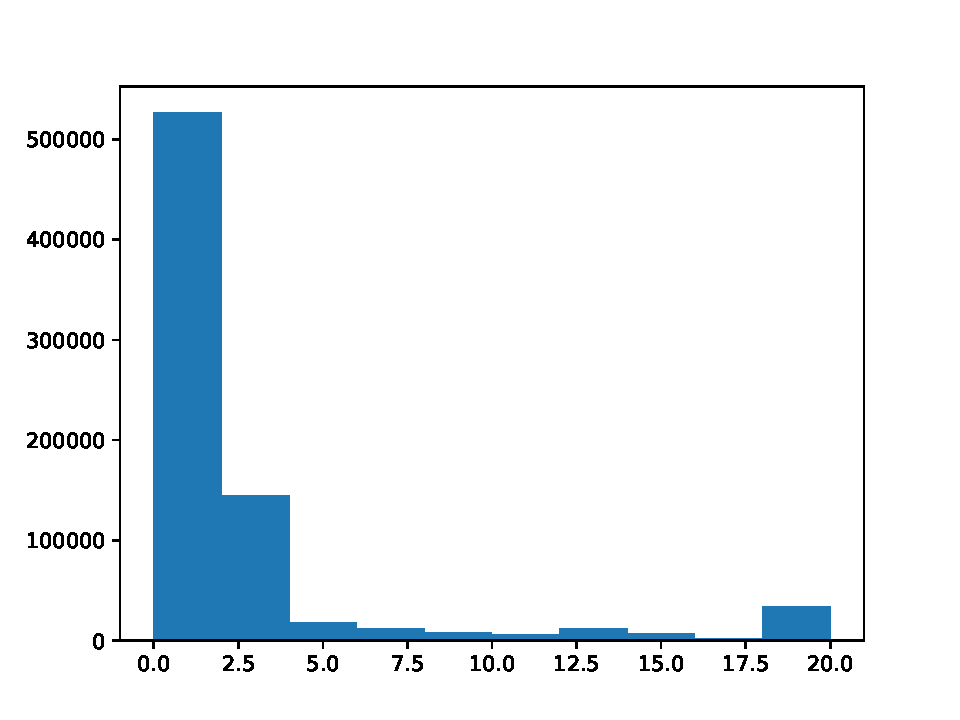
\includegraphics[width=1.11\linewidth]{MBSS/plot/Distribution/2022_01_cores.pdf} 
    %~ \caption{Cores - January 2022} 
    %~ \vspace{4ex}
  %~ \end{minipage}%%
  %~ \begin{minipage}[b]{0.5\linewidth}
    %~ \centering
    %~ 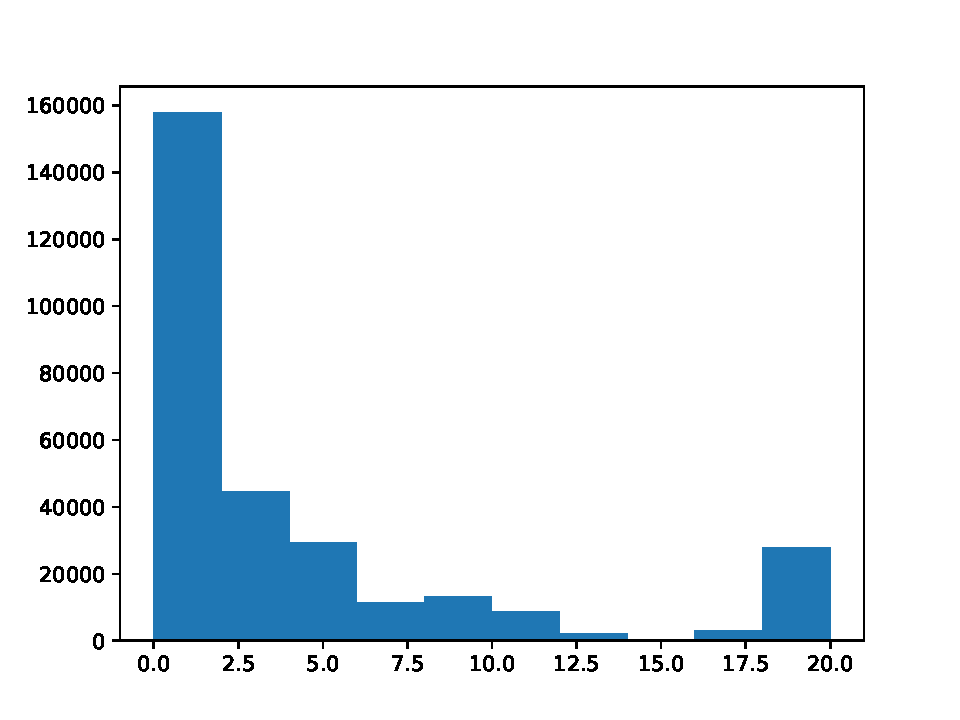
\includegraphics[width=1.11\linewidth]{MBSS/plot/Distribution/2022_02_cores.pdf} 
    %~ \caption{Cores - February 2022} 
    %~ \vspace{4ex}
  %~ \end{minipage} 
  %~ \begin{minipage}[b]{0.5\linewidth}
    %~ \centering
    %~ 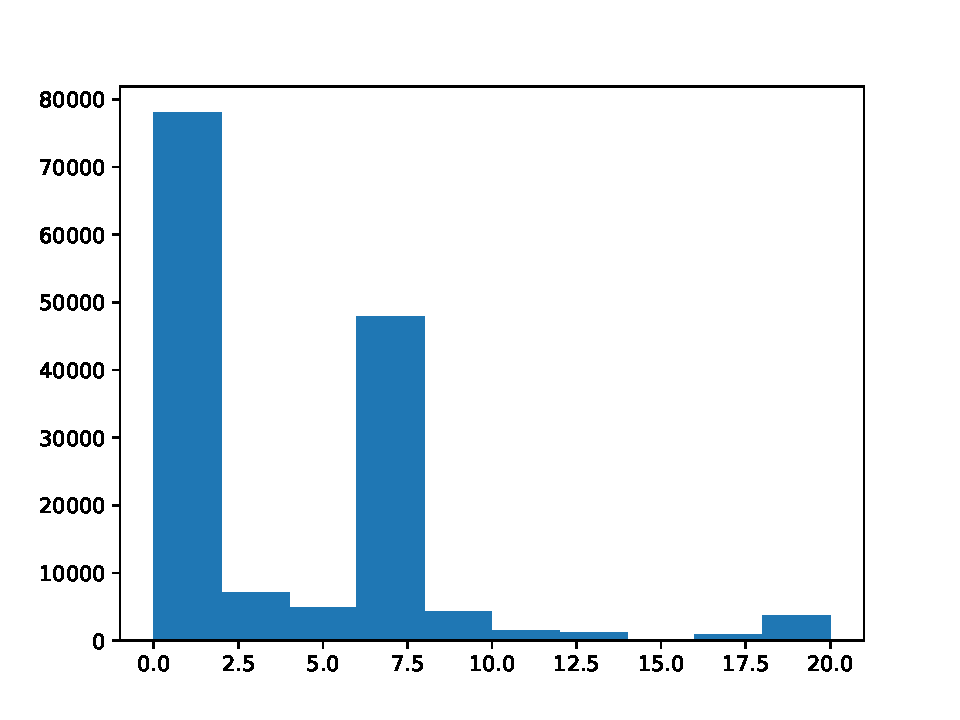
\includegraphics[width=1.11\linewidth]{MBSS/plot/Distribution/2022_03_cores.pdf} 
    %~ \caption{Cores - Mars 2022} 
    %~ \vspace{4ex}
  %~ \end{minipage}%% *
  %~ \begin{minipage}[b]{0.5\linewidth}
    %~ \centering
    %~ 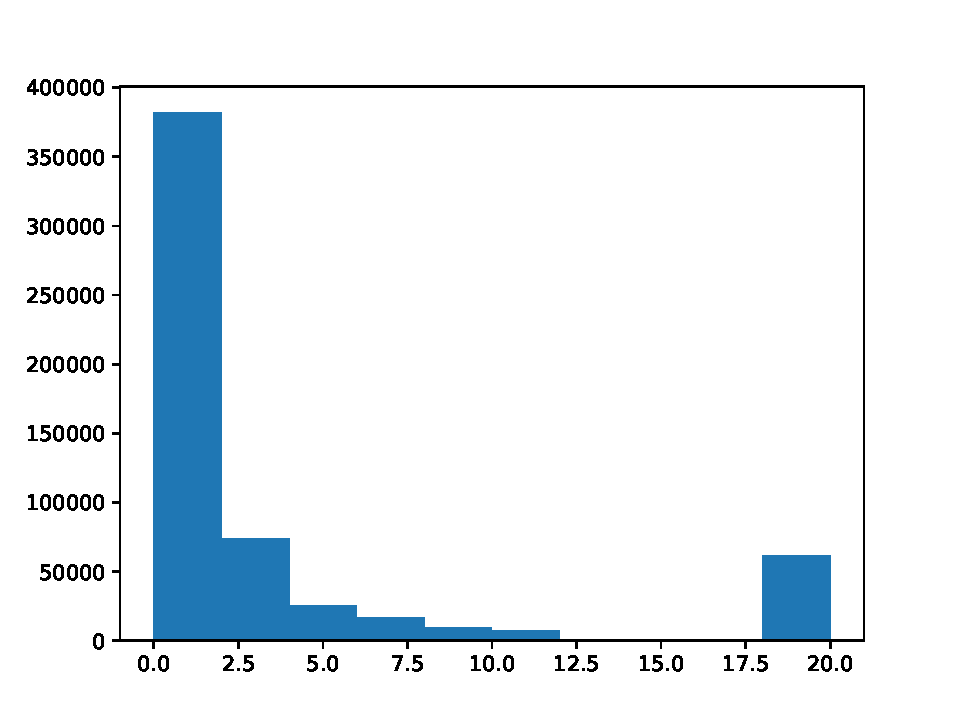
\includegraphics[width=1.11\linewidth]{MBSS/plot/Distribution/2021_12_cores.pdf} 
    %~ \caption{Cores - December 2021} 
    %~ \vspace{4ex}
  %~ \end{minipage}%%
%~ \end{figure}
%~ \begin{figure}[H] 
  %~ \begin{minipage}[b]{0.5\linewidth}
    %~ \centering
    %~ 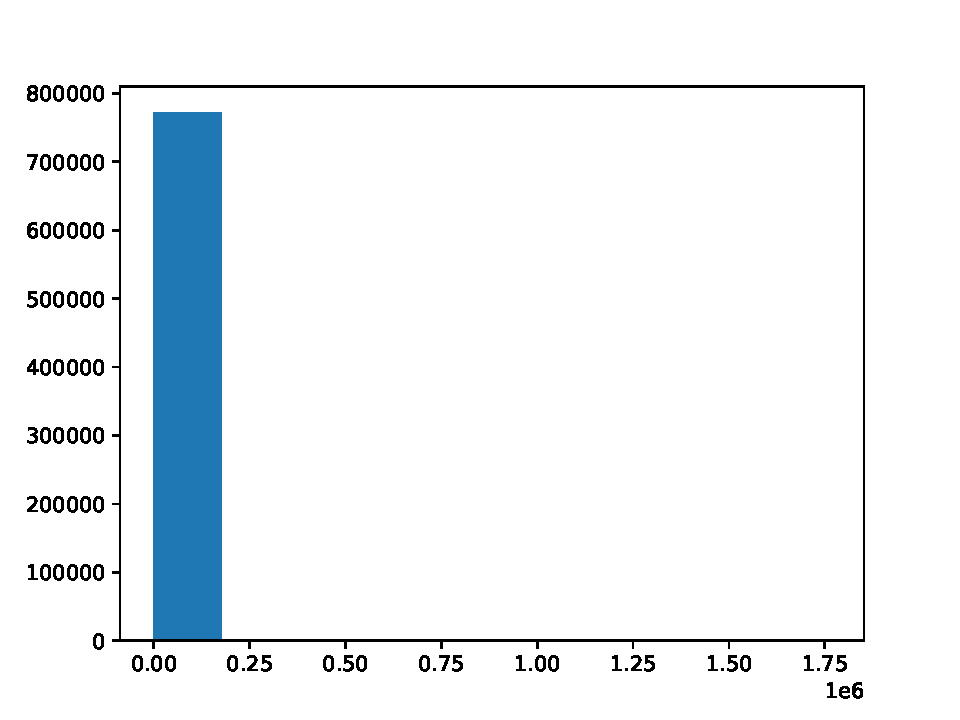
\includegraphics[width=1.11\linewidth]{MBSS/plot/Distribution/2022_01_delay.pdf} 
    %~ \caption{delay - January 2022} 
    %~ \vspace{4ex}
  %~ \end{minipage}%%
  %~ \begin{minipage}[b]{0.5\linewidth}
    %~ \centering
    %~ 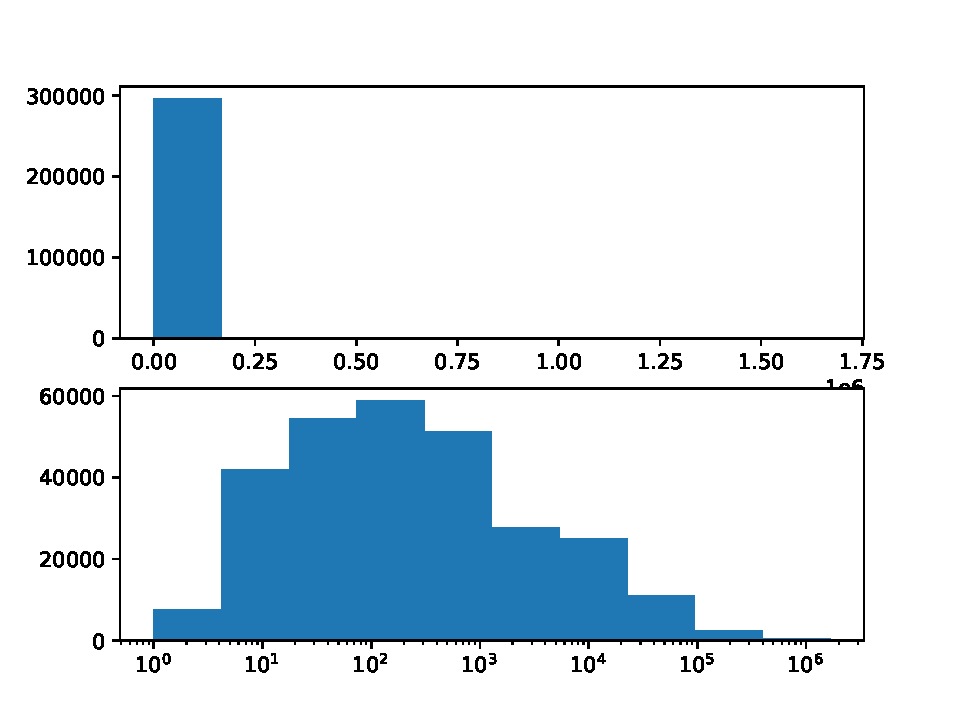
\includegraphics[width=1.11\linewidth]{MBSS/plot/Distribution/2022_02_delay.pdf} 
    %~ \caption{delay - February 2022} 
    %~ \vspace{4ex}
  %~ \end{minipage} 
  %~ \begin{minipage}[b]{0.5\linewidth}
    %~ \centering
    %~ 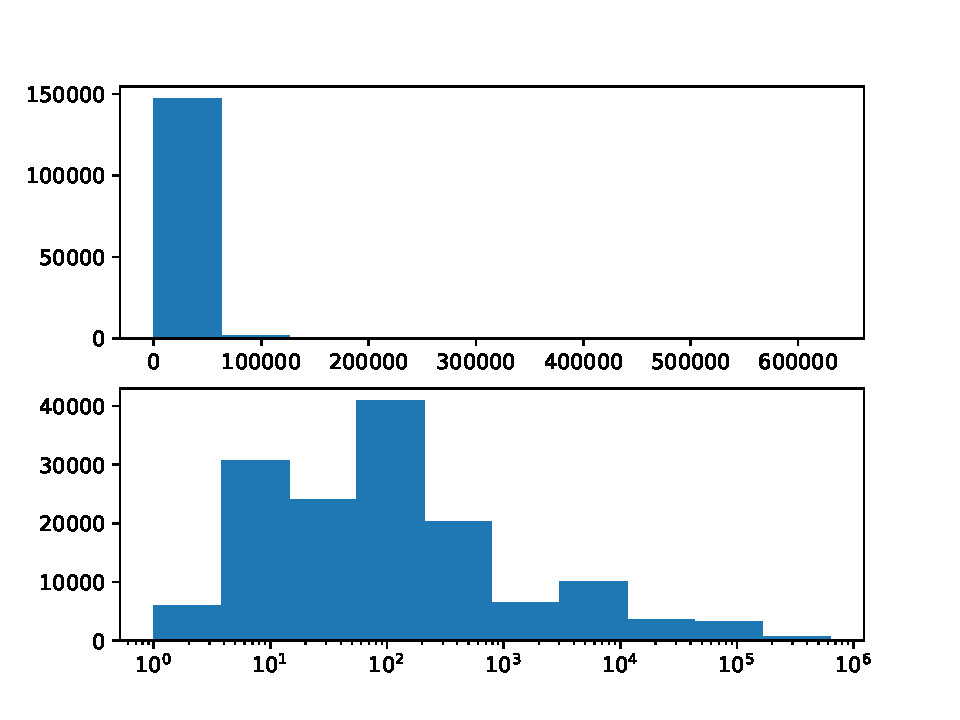
\includegraphics[width=1.11\linewidth]{MBSS/plot/Distribution/2022_03_delay.pdf} 
    %~ \caption{delay - Mars 2022} 
    %~ \vspace{4ex}
  %~ \end{minipage}%% 
    %~ \begin{minipage}[b]{0.5\linewidth}
    %~ \centering
    %~ 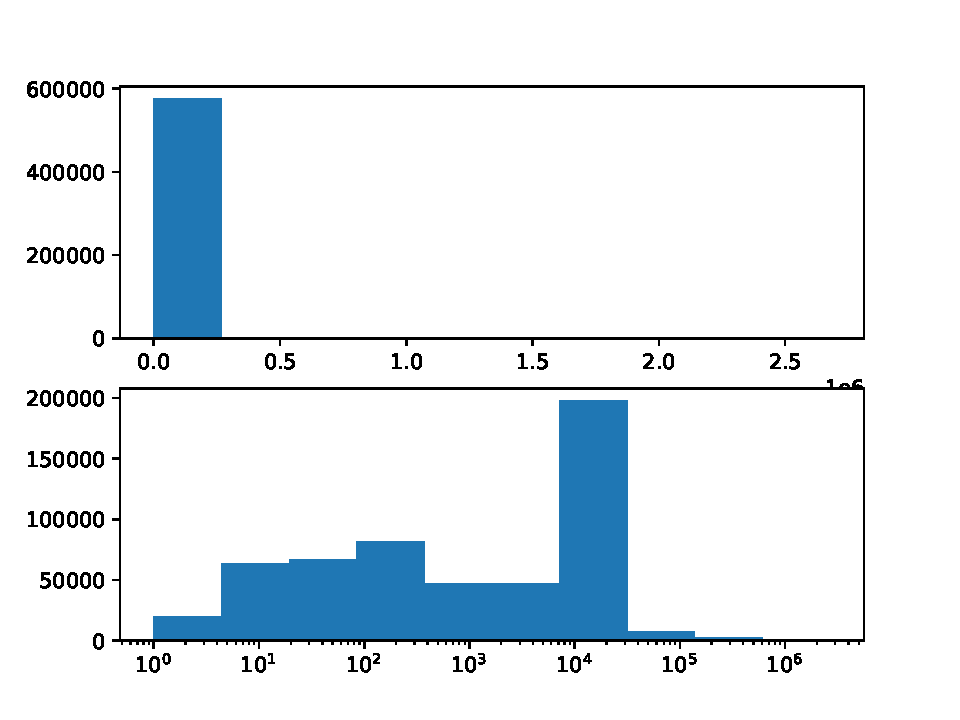
\includegraphics[width=1.11\linewidth]{MBSS/plot/Distribution/2021_12_delay.pdf} 
    %~ \caption{delay - December 2021} 
    %~ \vspace{4ex}
  %~ \end{minipage}%%
%~ \end{figure}
%~ \begin{figure}[H] 
  %~ \begin{minipage}[b]{0.5\linewidth}
    %~ \centering
    %~ 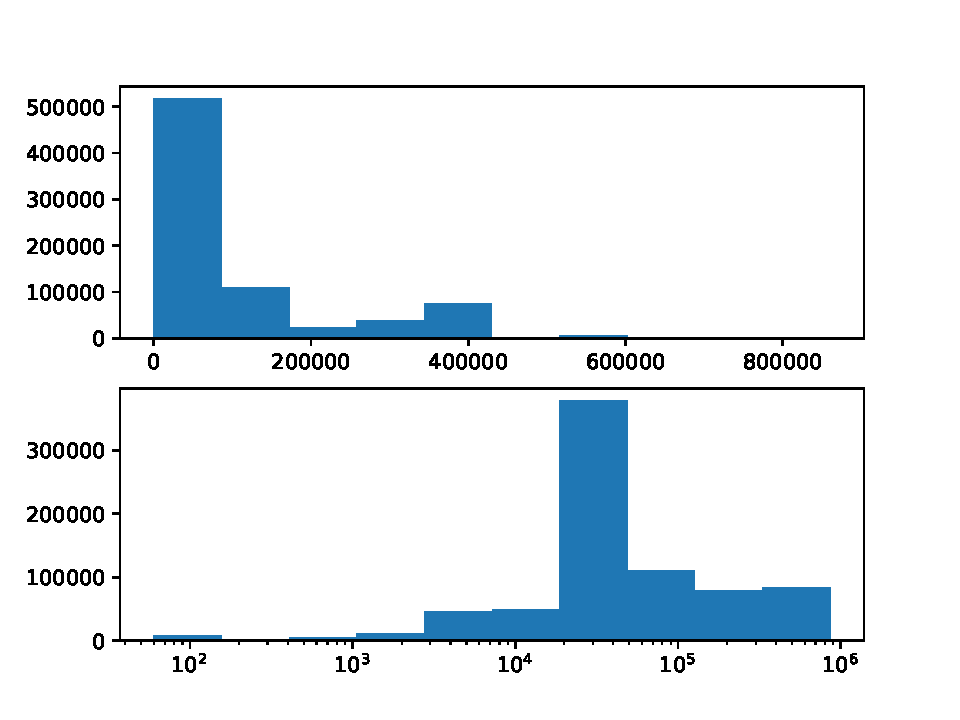
\includegraphics[width=1.11\linewidth]{MBSS/plot/Distribution/2022_01_walltime.pdf} 
    %~ \caption{walltime - January 2022} 
    %~ \vspace{4ex}
  %~ \end{minipage}%%
  %~ \begin{minipage}[b]{0.5\linewidth}
    %~ \centering
    %~ 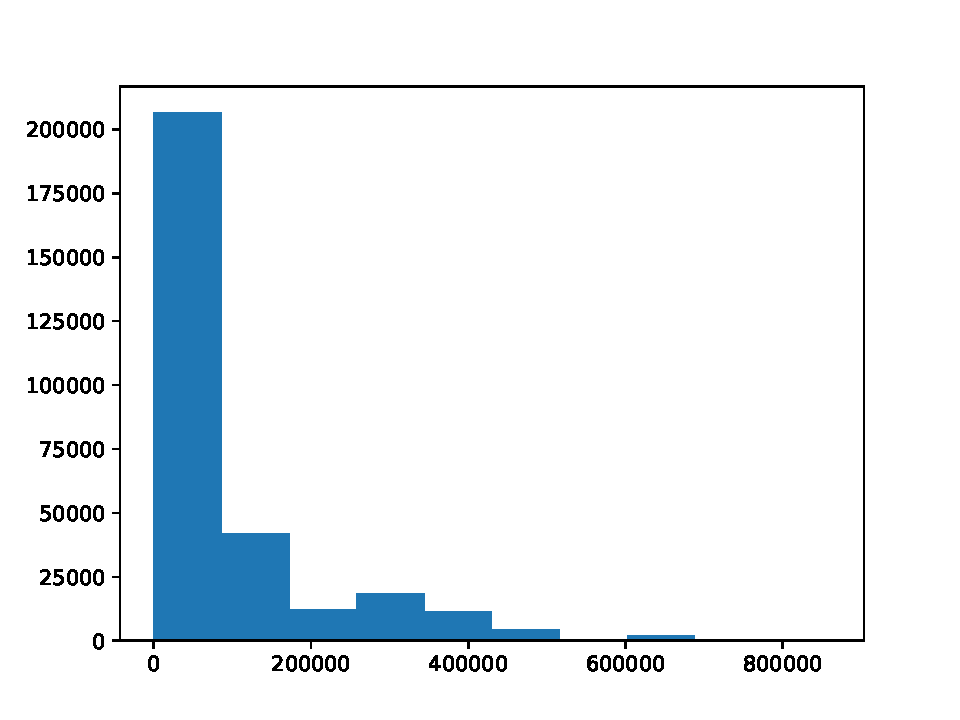
\includegraphics[width=1.11\linewidth]{MBSS/plot/Distribution/2022_02_walltime.pdf} 
    %~ \caption{walltime - February 2022} 
    %~ \vspace{4ex}
  %~ \end{minipage} 
  %~ \begin{minipage}[b]{0.5\linewidth}
    %~ \centering
    %~ 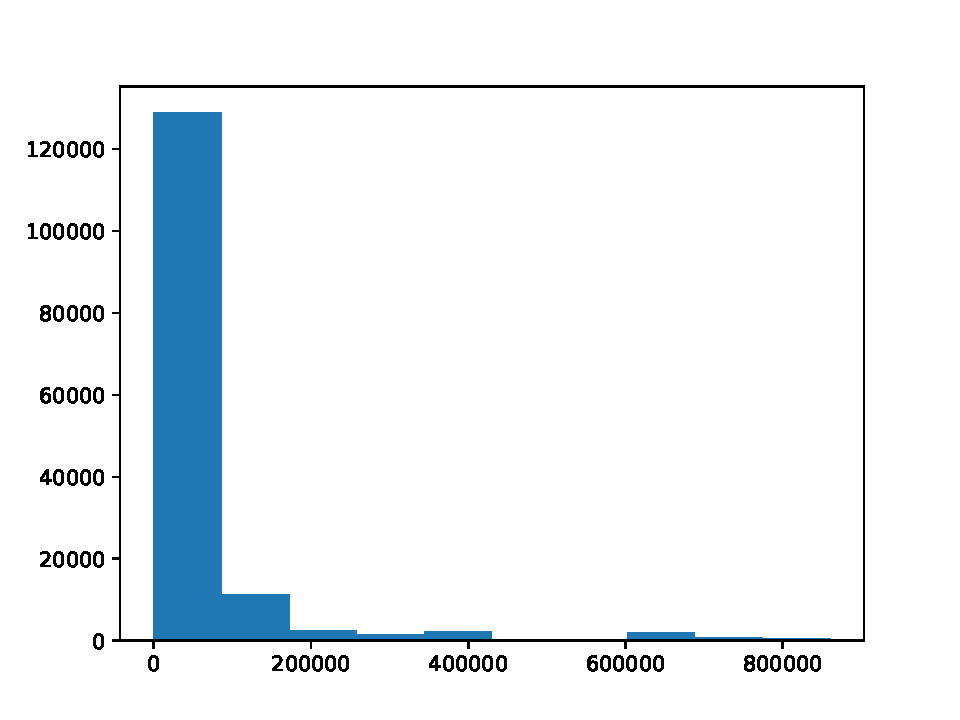
\includegraphics[width=1.11\linewidth]{MBSS/plot/Distribution/2022_03_walltime.pdf} 
    %~ \caption{walltime - Mars 2022} 
    %~ \vspace{4ex}
  %~ \end{minipage}%% 
  %~ \begin{minipage}[b]{0.5\linewidth}
    %~ \centering
    %~ 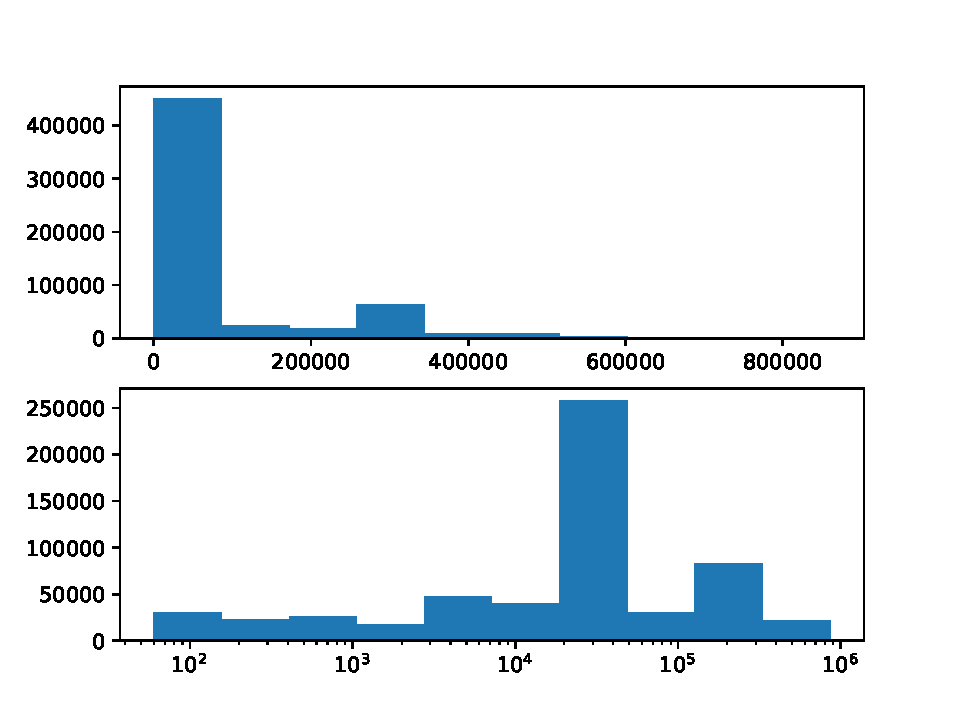
\includegraphics[width=1.11\linewidth]{MBSS/plot/Distribution/2021_12_walltime.pdf} 
    %~ \caption{walltime - Decembre 2021} 
    %~ \vspace{4ex}
  %~ \end{minipage}%%
%~ \end{figure}

\section{Gantt charts}
\begin{figure}[H] 
  \begin{minipage}[b]{0.5\linewidth}
    \centering
    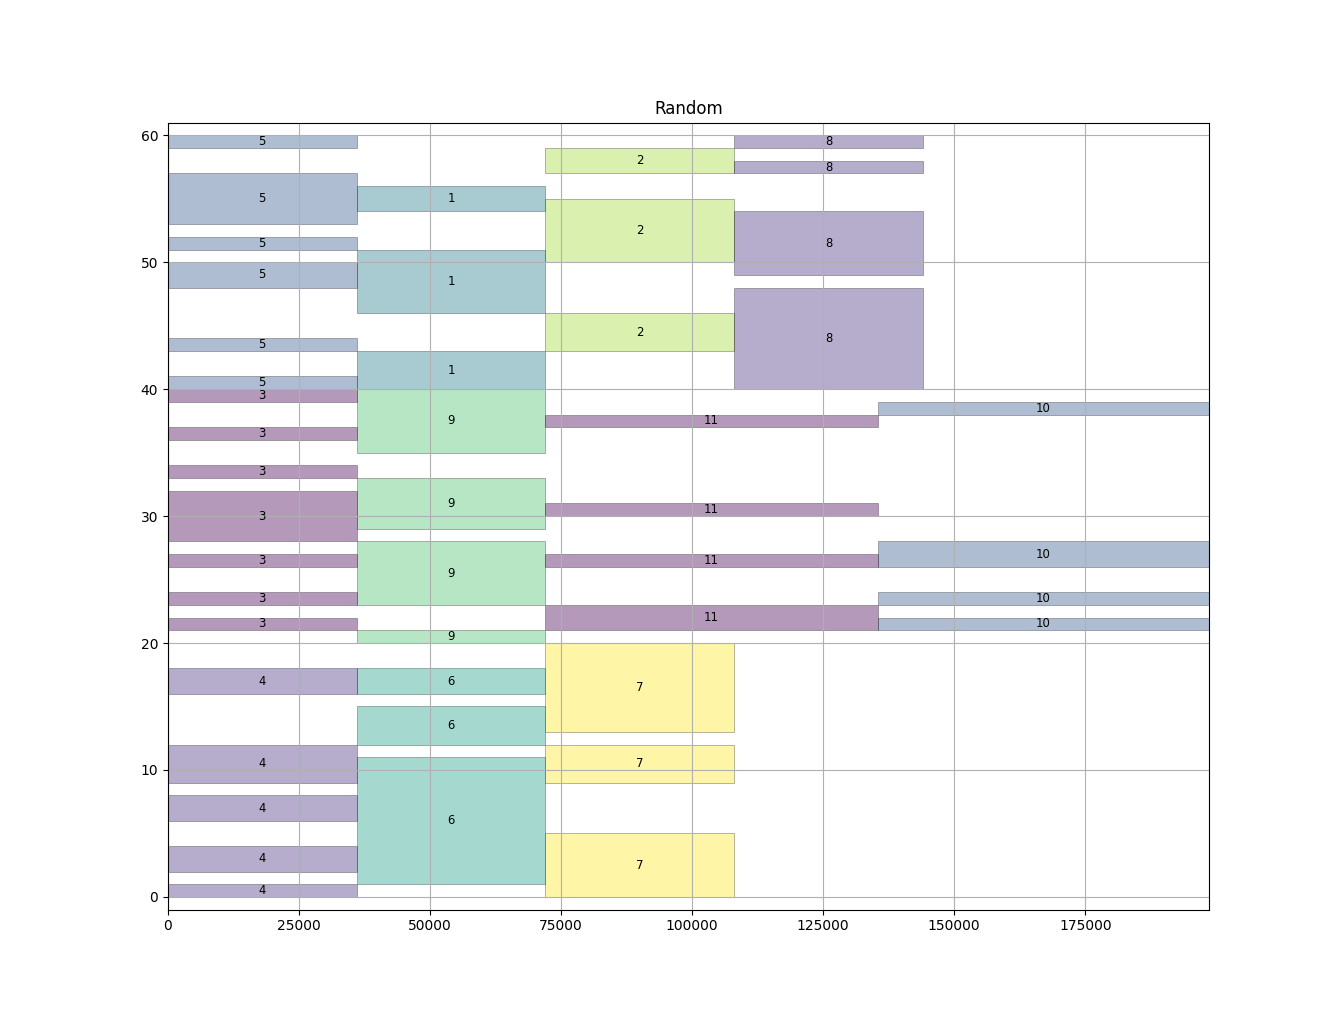
\includegraphics[width=1.11\linewidth]{MBSS/plot/Gantt_charts/test/Random.png} 
    \caption{Random - May 5} 
    \vspace{4ex}
  \end{minipage}%%
  \begin{minipage}[b]{0.5\linewidth}
    \centering
    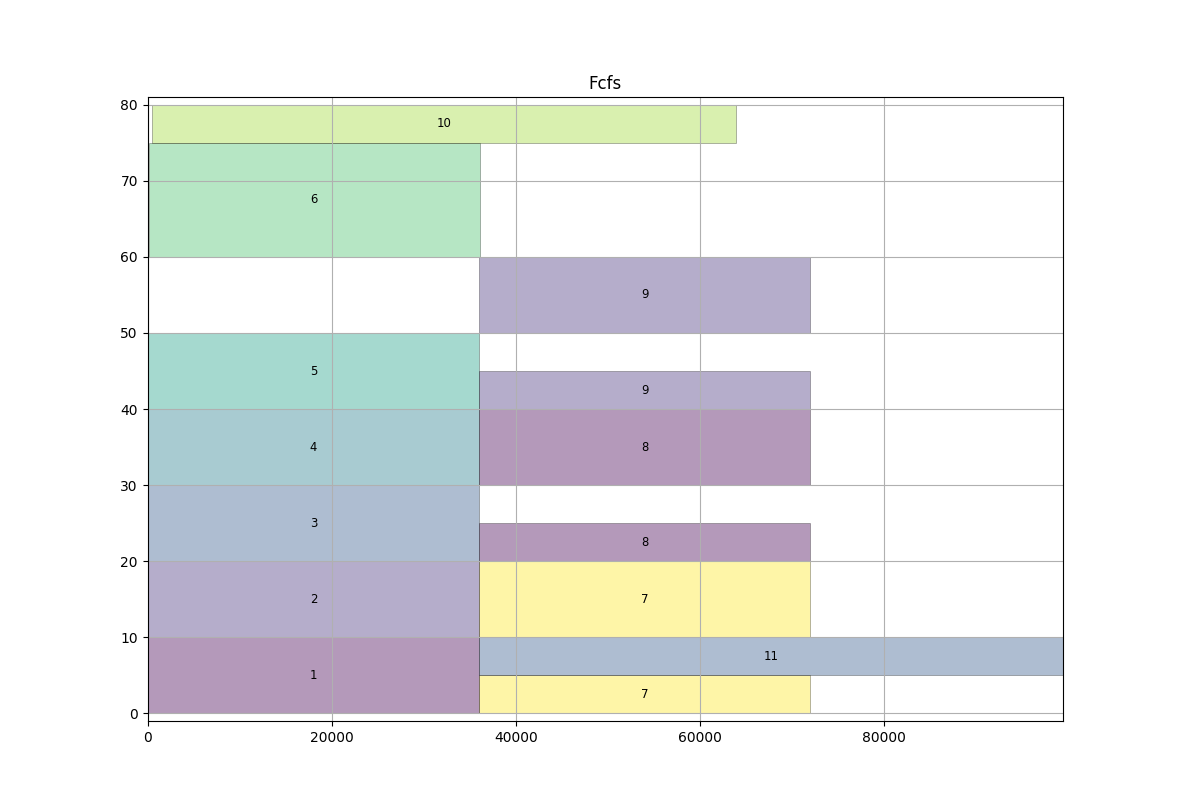
\includegraphics[width=1.11\linewidth]{MBSS/plot/Gantt_charts/test/Fcfs.png} 
    \caption{FCFS - May 5} 
    \vspace{4ex}
  \end{minipage}
  \begin{minipage}[b]{0.5\linewidth}
    \centering
    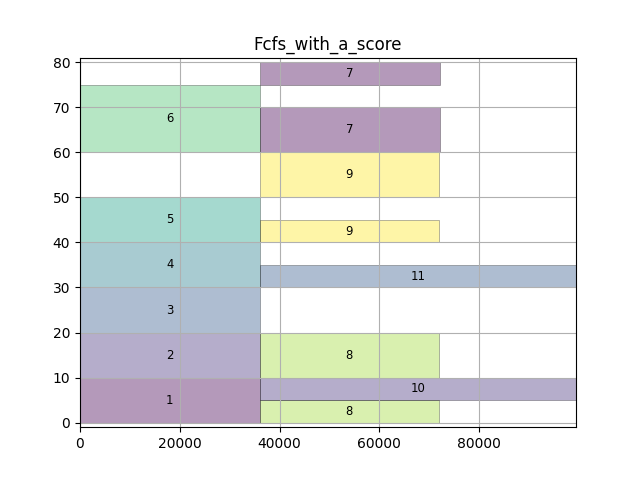
\includegraphics[width=1.11\linewidth]{MBSS/plot/Gantt_charts/test/Fcfs_with_a_score.png} 
    \caption{FCFS with a score- May 5} 
    \vspace{4ex}
  \end{minipage}%%
  \begin{minipage}[b]{0.5\linewidth}
    \centering
    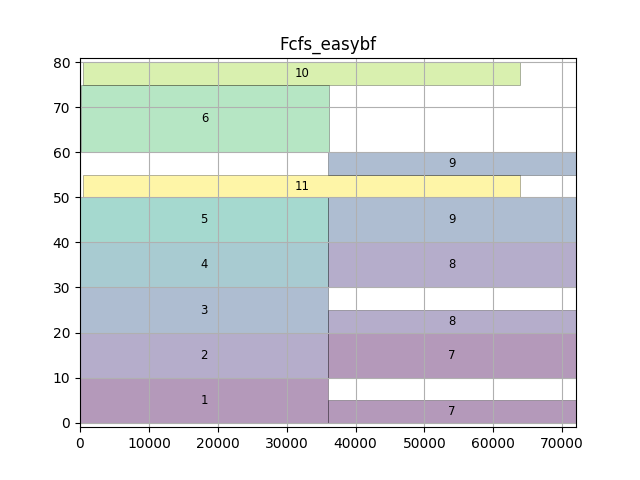
\includegraphics[width=1.11\linewidth]{MBSS/plot/Gantt_charts/test/Fcfs_easybf.png} 
    \caption{FCFS + Easy Bf - May 5} 
    \vspace{4ex}
  \end{minipage}
  \begin{minipage}[b]{0.5\linewidth}
    \centering
    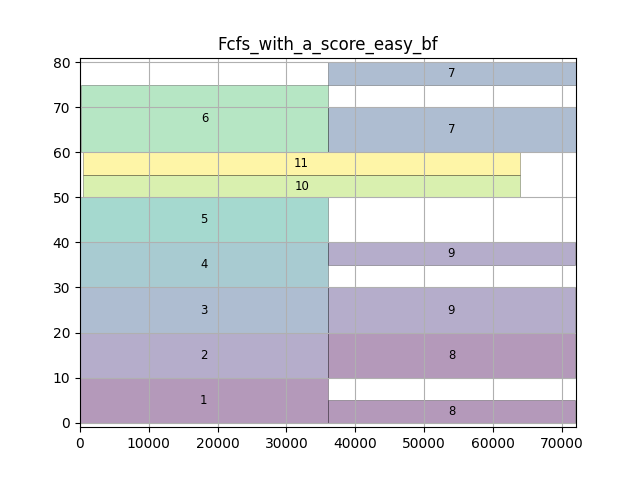
\includegraphics[width=1.11\linewidth]{MBSS/plot/Gantt_charts/test/Fcfs_with_a_score_easy_bf.png} 
    \caption{FCFS with a score + Easy Bf - May 5} 
    \vspace{4ex}
  \end{minipage}%%
  \begin{minipage}[b]{0.5\linewidth}
    \centering
    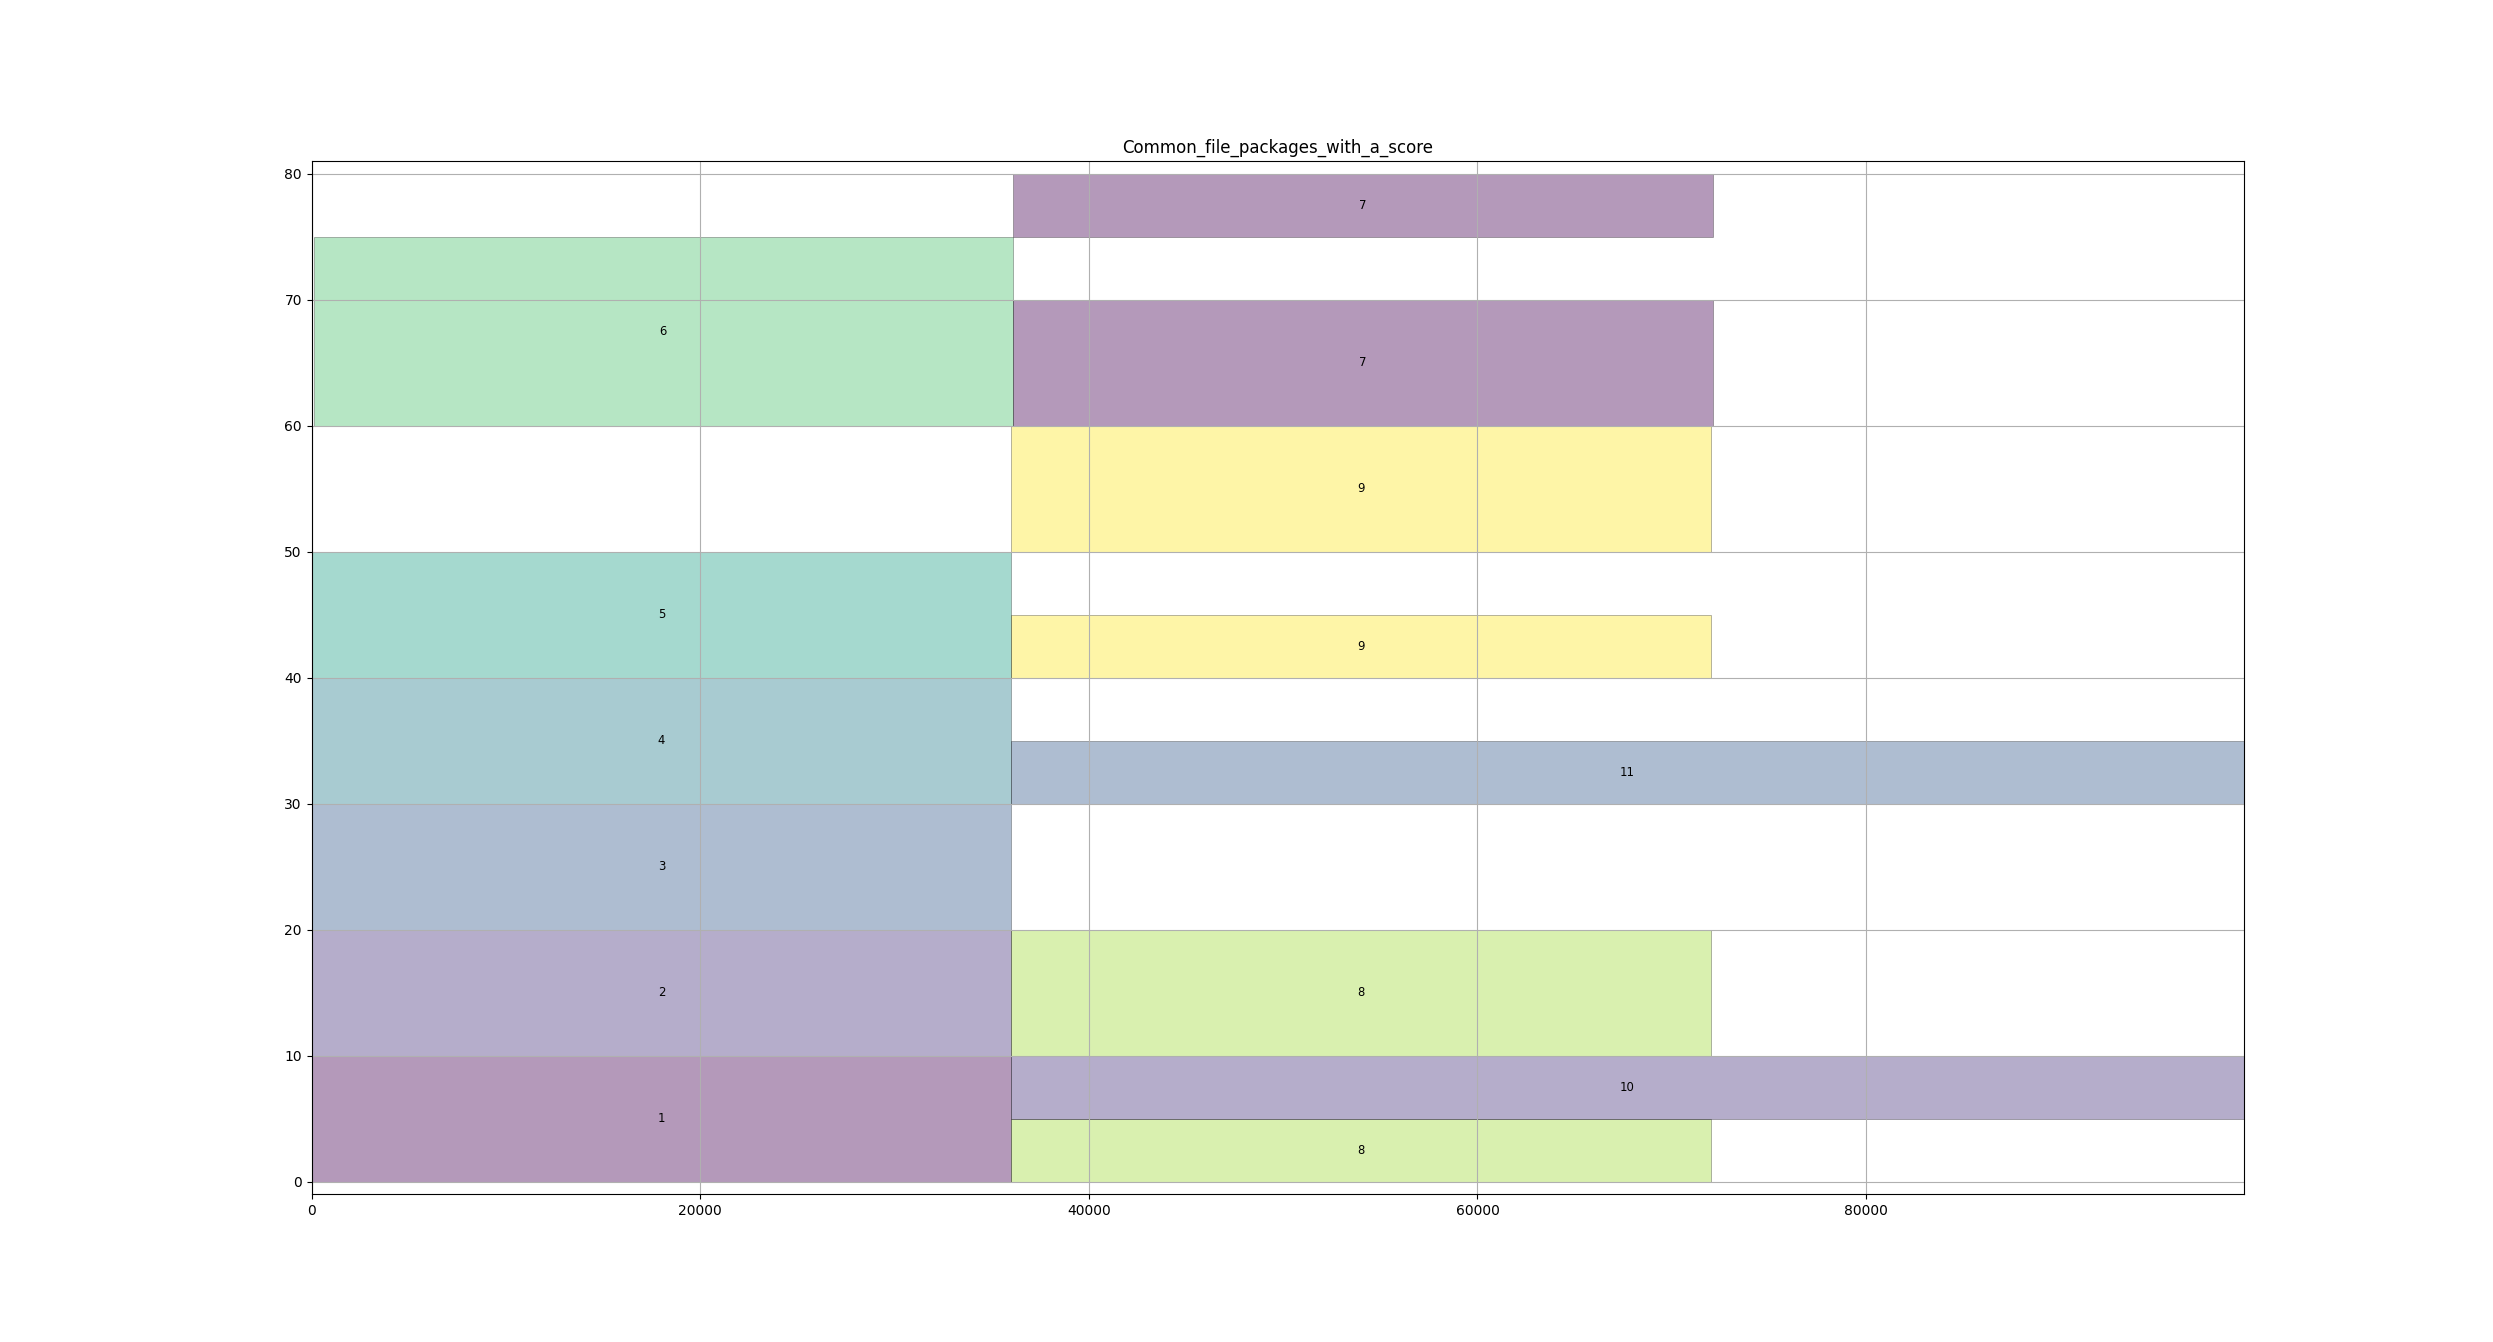
\includegraphics[width=1.11\linewidth]{MBSS/plot/Gantt_charts/test/Common_file_packages_with_a_score.png} 
    \caption{Common file packages with a score - May 12} 
    \vspace{4ex}
  \end{minipage}
\end{figure}

\section{Experiments}
		
	\subsection{1 day and full cluster}
	\begin{figure}[H]\centering
	\begin{subfigure}[b]{0.4\linewidth}\centering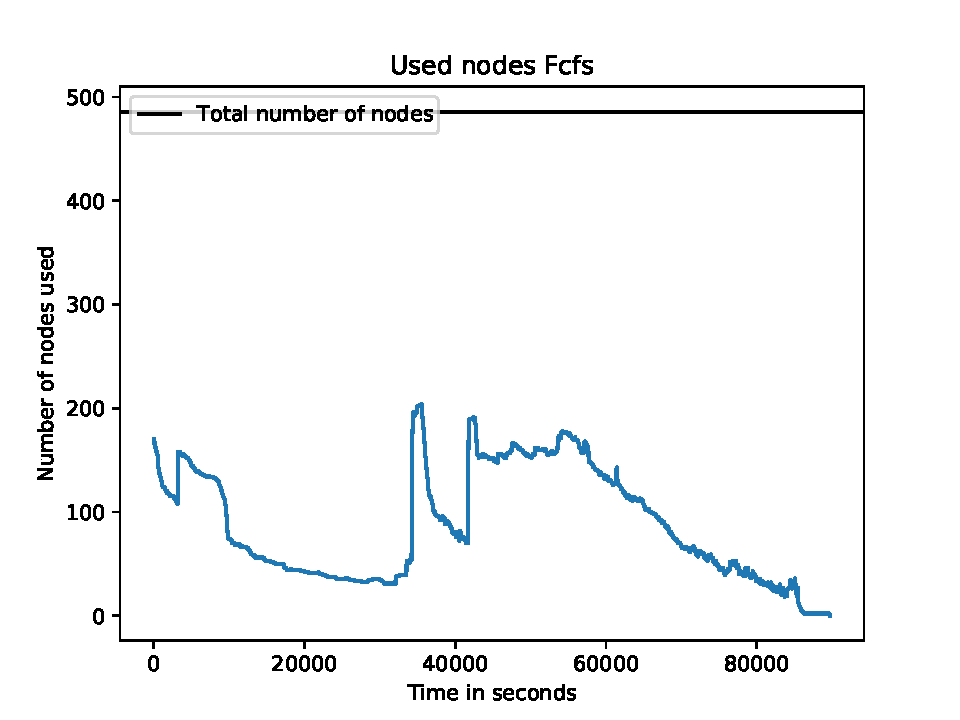
\includegraphics[width=1\linewidth]{MBSS/plot/2022-03-14->2022-03-14_Fcfs_Used_nodes_450_128_32_256_4_1024.pdf}\caption{Used nodes}\end{subfigure}
	\begin{subfigure}[b]{0.4\linewidth}\centering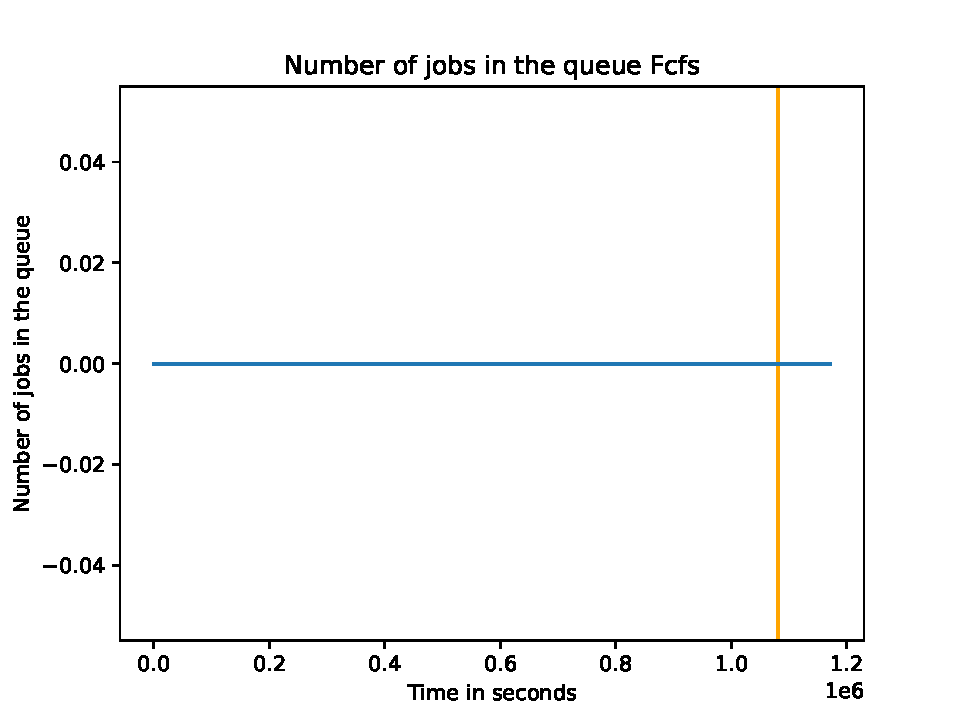
\includegraphics[width=1\linewidth]{MBSS/plot/2022-03-14->2022-03-14_Fcfs_Nb_scheduled_jobs_450_128_32_256_4_1024.pdf}\caption{Jobs in queue}\end{subfigure}
	\caption{Workload 2022-03-14-2022-03-14 - Cluster usage - Full cluster - May 20}\end{figure}
	
	\subsection{2 days and full cluster}
	\begin{figure}[H]\centering
	\begin{subfigure}[b]{0.4\linewidth}\centering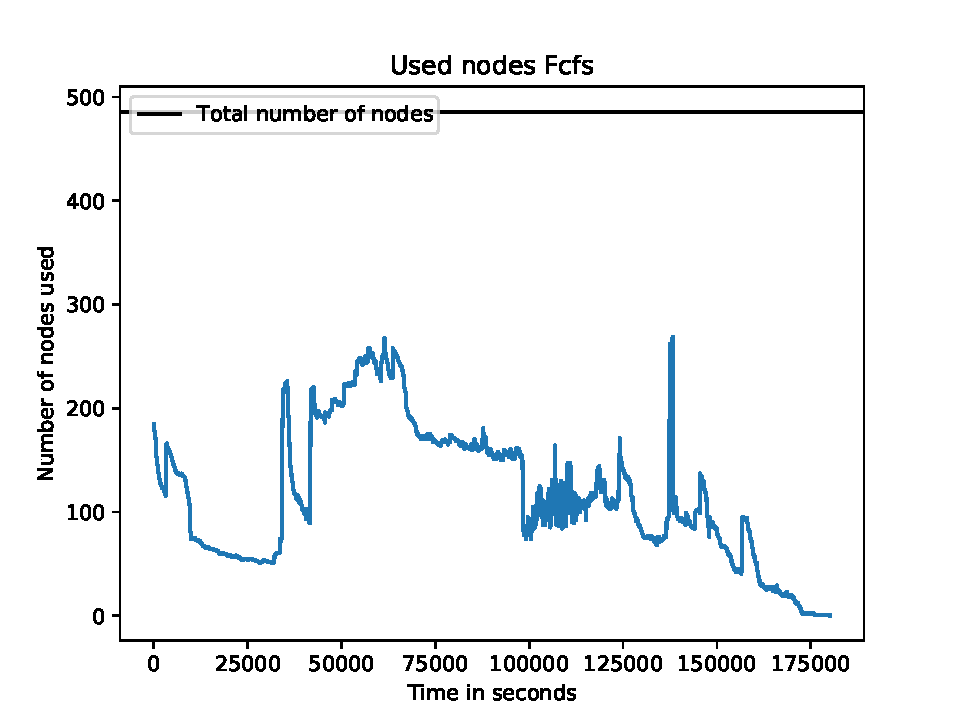
\includegraphics[width=1\linewidth]{MBSS/plot/2022-03-14->2022-03-15_Fcfs_Used_nodes_450_128_32_256_4_1024.pdf}\caption{Used nodes}\end{subfigure}
	\begin{subfigure}[b]{0.4\linewidth}\centering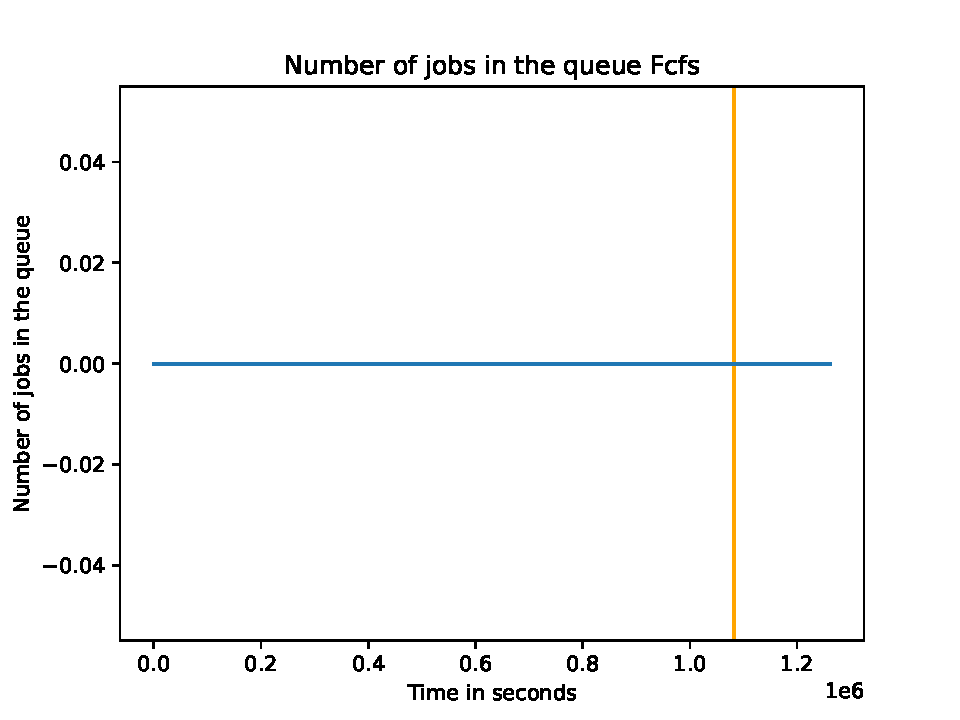
\includegraphics[width=1\linewidth]{MBSS/plot/2022-03-14->2022-03-15_Fcfs_Nb_scheduled_jobs_450_128_32_256_4_1024.pdf}\caption{Jobs in queue}\end{subfigure}
	\caption{Workload 2022-03-14-2022-03-15 - Cluster usage - Full cluster - May 20}\end{figure}
	
	\subsection{3 days and full cluster}
	\begin{figure}[H]\centering
	\begin{subfigure}[b]{0.4\linewidth}\centering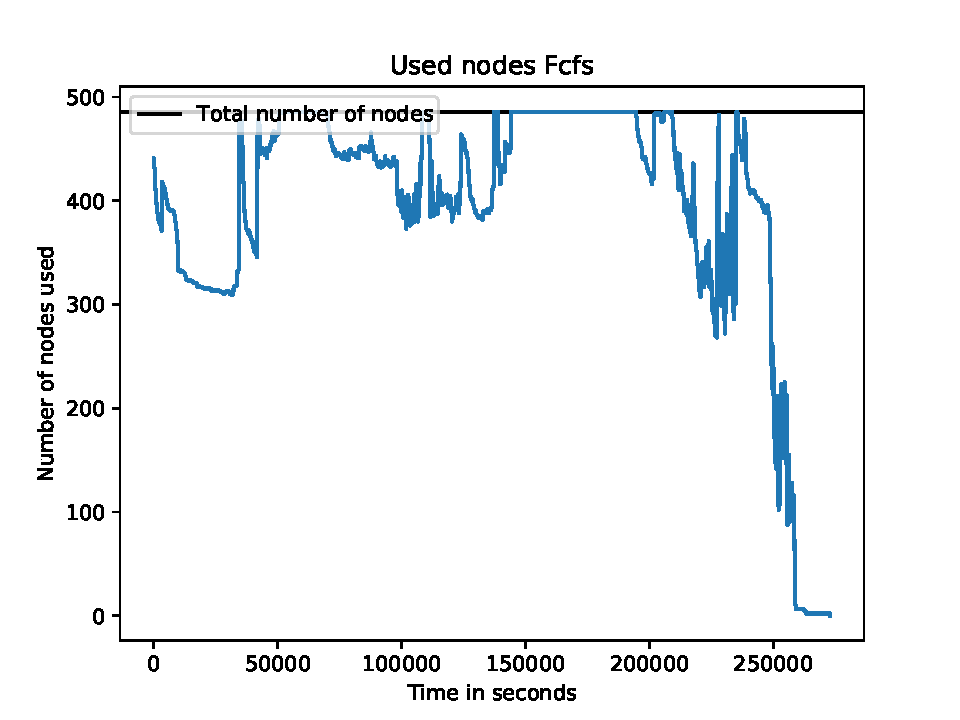
\includegraphics[width=1\linewidth]{MBSS/plot/2022-03-14->2022-03-16_Fcfs_Used_nodes_450_128_32_256_4_1024.pdf}\caption{Used nodes}\end{subfigure}
	\begin{subfigure}[b]{0.4\linewidth}\centering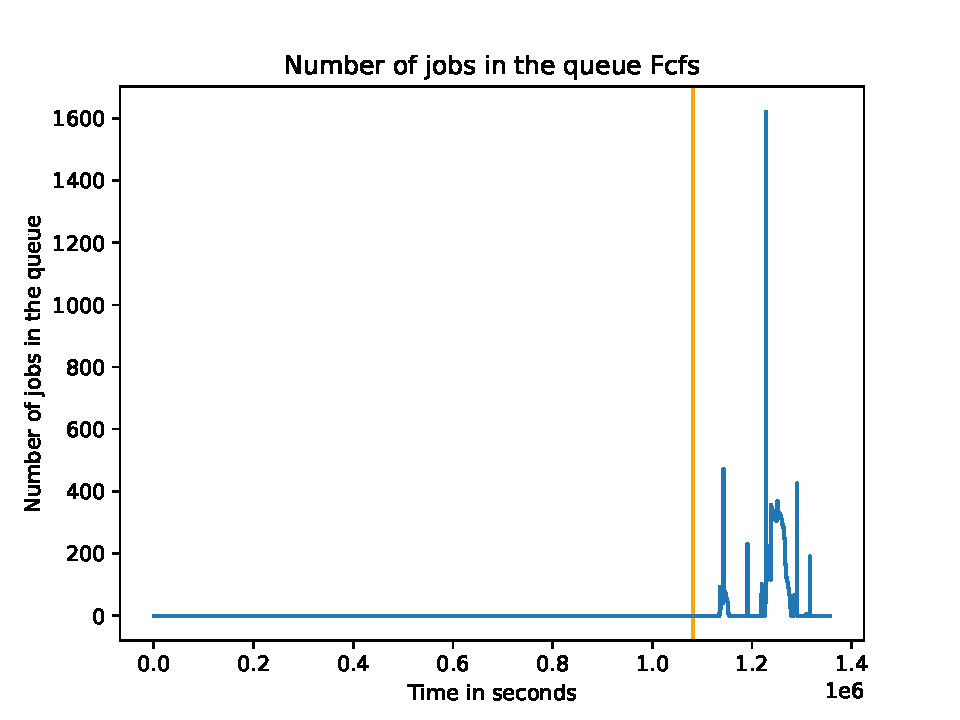
\includegraphics[width=1\linewidth]{MBSS/plot/2022-03-14->2022-03-16_Fcfs_Nb_scheduled_jobs_450_128_32_256_4_1024.pdf}\caption{Jobs in queue}\end{subfigure}
	\caption{Workload 2022-03-14-2022-03-16 - Cluster usage - Full cluster - May 20}\end{figure}
	
	\subsection{1 day and 1/4 cluster}
	\begin{figure}[H]\begin{subfigure}[b]{0.4\linewidth}\centering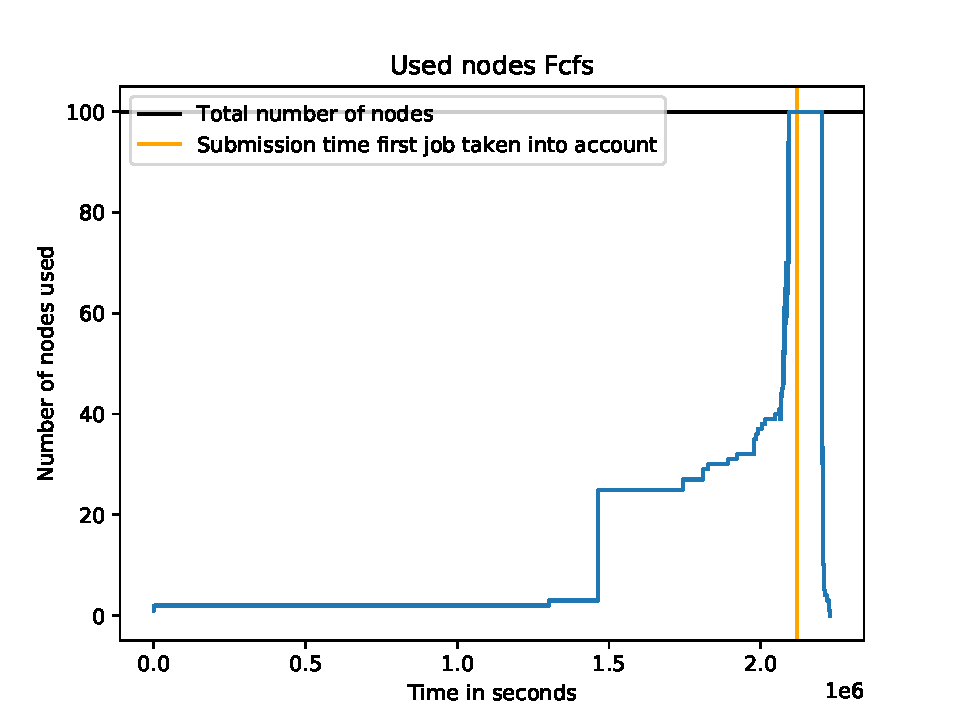
\includegraphics[width=1\linewidth]{MBSS/plot/2022-03-26->2022-03-26_Fcfs_Used_nodes_95_128_4_256_1_1024.pdf}\caption{Used nodes}\end{subfigure}
	\begin{subfigure}[b]{0.4\linewidth}\centering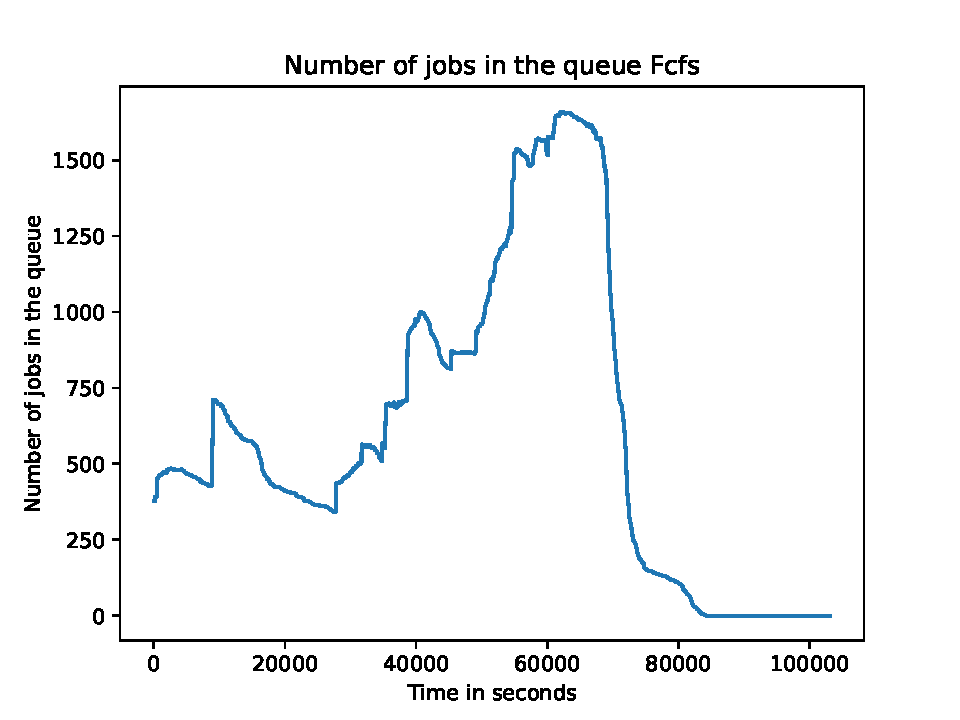
\includegraphics[width=1\linewidth]{MBSS/plot/2022-03-26->2022-03-26_Fcfs_Nb_scheduled_jobs_95_128_4_256_1_1024.pdf}\caption{Jobs in queue}\end{subfigure}\caption{Workload 2022-03-26 - Cluster usage - 1/4 cluster - May 30}\end{figure}
		
	\begin{figure}[H]\centering
	\begin{subfigure}[b]{0.4\linewidth}\centering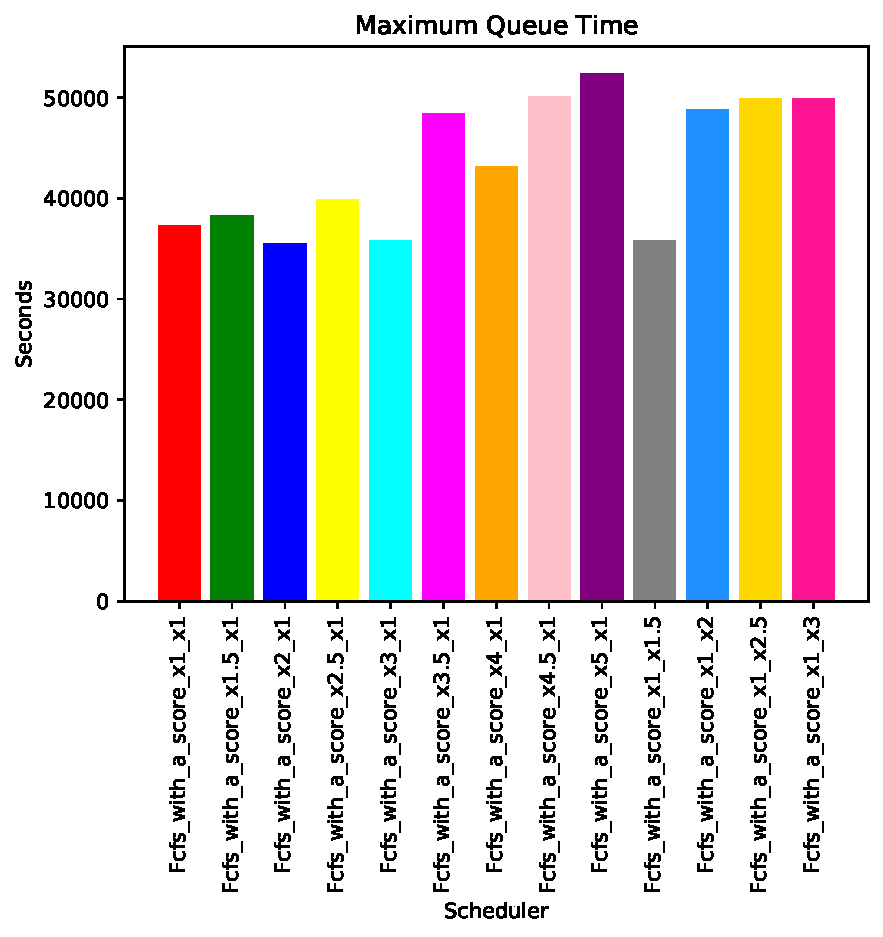
\includegraphics[width=1\linewidth]{MBSS/plot/FCFS_Score_2022-03-26->2022-03-26_Maximum_queue_time_95_128_4_256_1_1024.pdf}\caption{Maximum queue time}\end{subfigure}
	\begin{subfigure}[b]{0.4\linewidth}\centering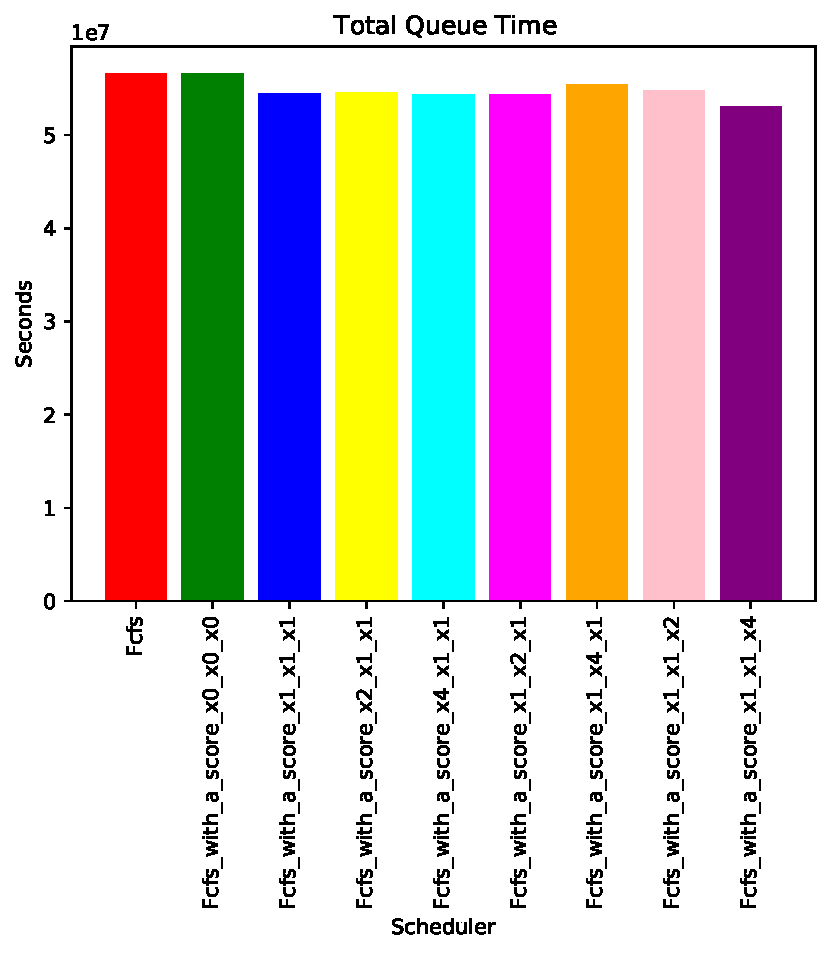
\includegraphics[width=1\linewidth]{MBSS/plot/FCFS_Score_2022-03-26->2022-03-26_Total_queue_time_95_128_4_256_1_1024.pdf}\caption{Total queue time}\end{subfigure}
	\begin{subfigure}[b]{0.4\linewidth}\centering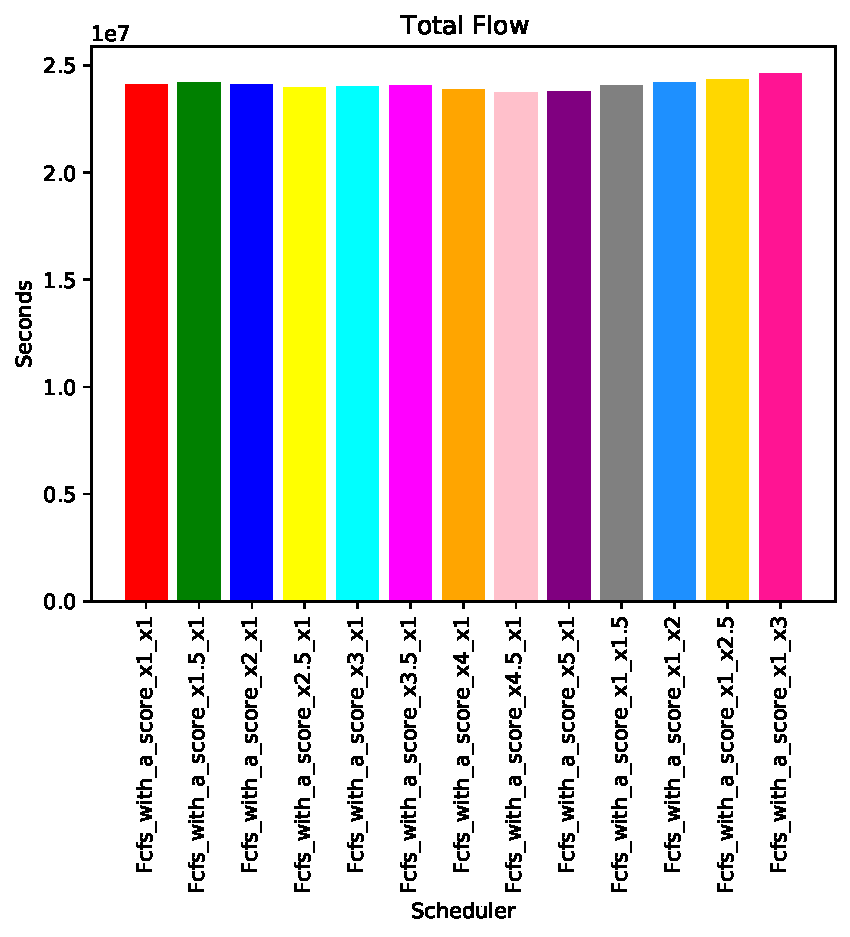
\includegraphics[width=1\linewidth]{MBSS/plot/FCFS_Score_2022-03-26->2022-03-26_Total_flow_95_128_4_256_1_1024.pdf}\caption{Total flow}\end{subfigure}
	\begin{subfigure}[b]{0.4\linewidth}\centering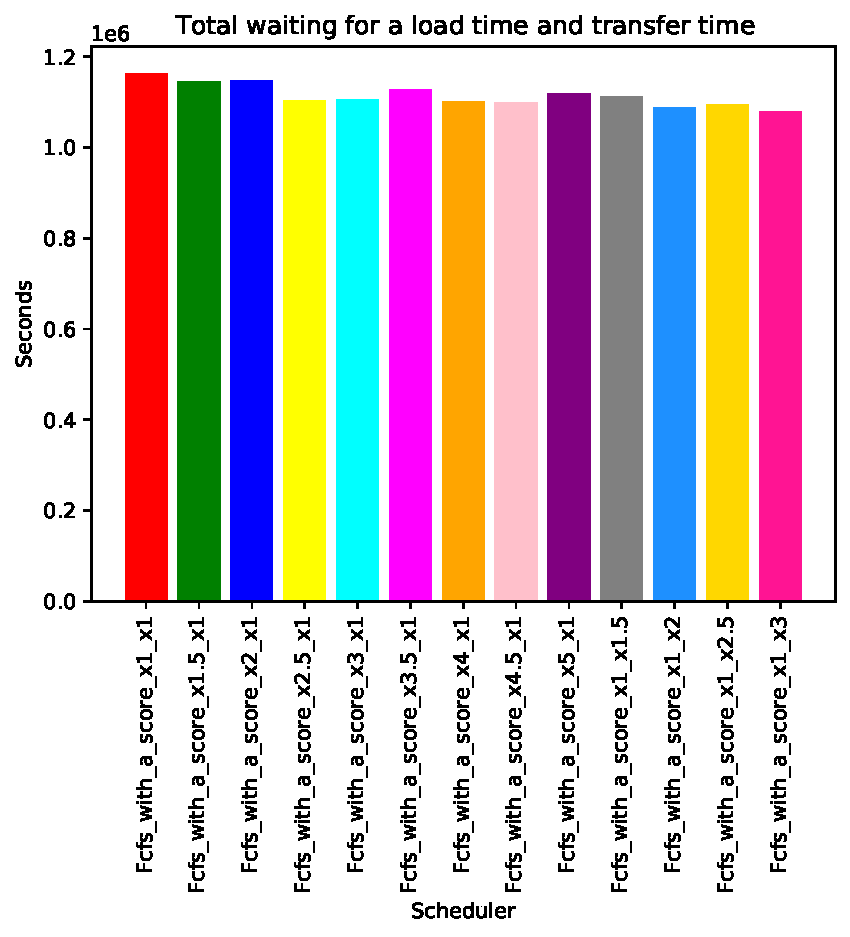
\includegraphics[width=1\linewidth]{MBSS/plot/FCFS_Score_2022-03-26->2022-03-26_Total_waiting_for_a_load_time_and_transfer_time_95_128_4_256_1_1024.pdf}\caption{Waiting for a load and transfer time}\end{subfigure}\caption{Workload 2022-03-26 - Performance on FCFS with a score, no constraint on files sizes - 1/4 cluster - May 30}\end{figure}
	
	\begin{figure}[H]\centering
	\begin{subfigure}[b]{0.4\linewidth}\centering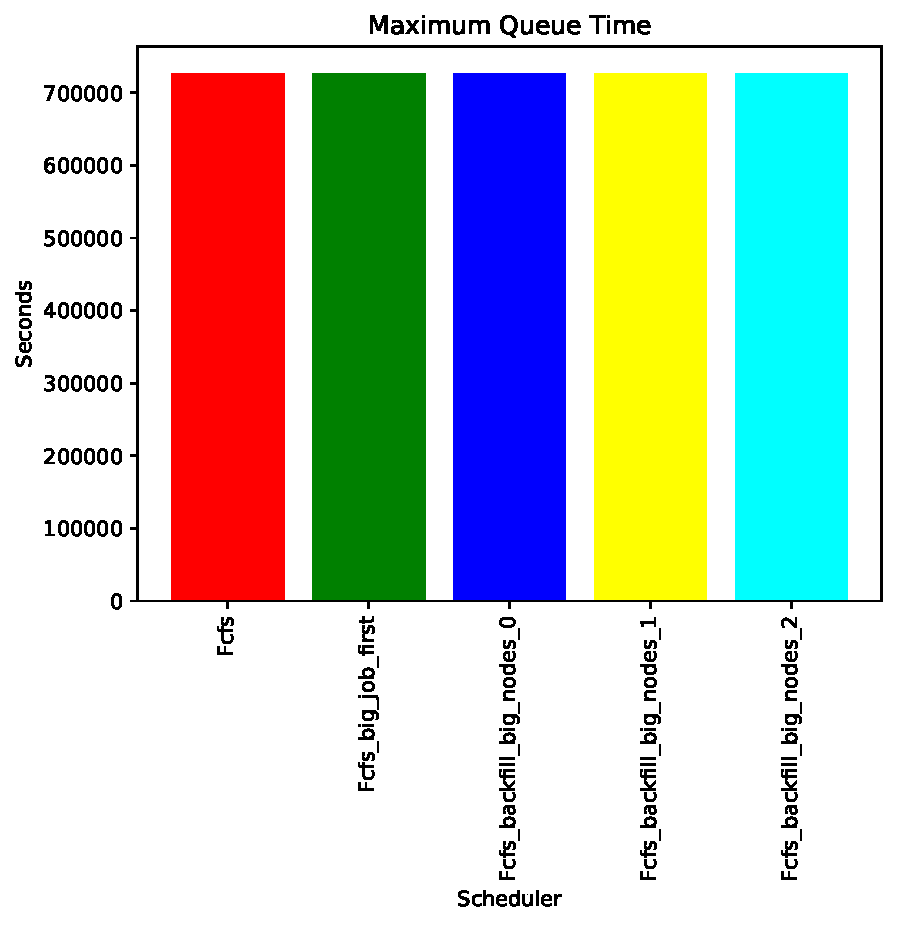
\includegraphics[width=1\linewidth]{MBSS/plot/Size_Constraint_2022-03-26->2022-03-26_classic_Maximum_queue_time_95_128_4_256_1_1024.pdf}\caption{Maximum queue time}\end{subfigure}
	\begin{subfigure}[b]{0.4\linewidth}\centering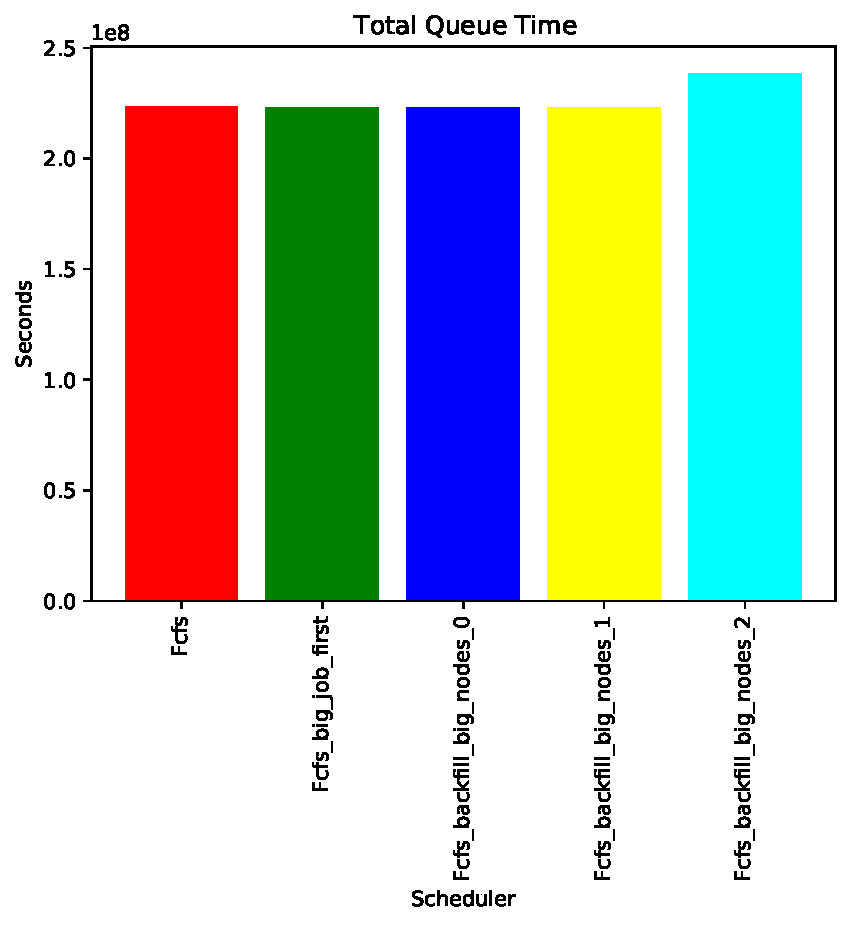
\includegraphics[width=1\linewidth]{MBSS/plot/Size_Constraint_2022-03-26->2022-03-26_classic_Total_queue_time_95_128_4_256_1_1024.pdf}\caption{Total queue time}\end{subfigure}
	\begin{subfigure}[b]{0.4\linewidth}\centering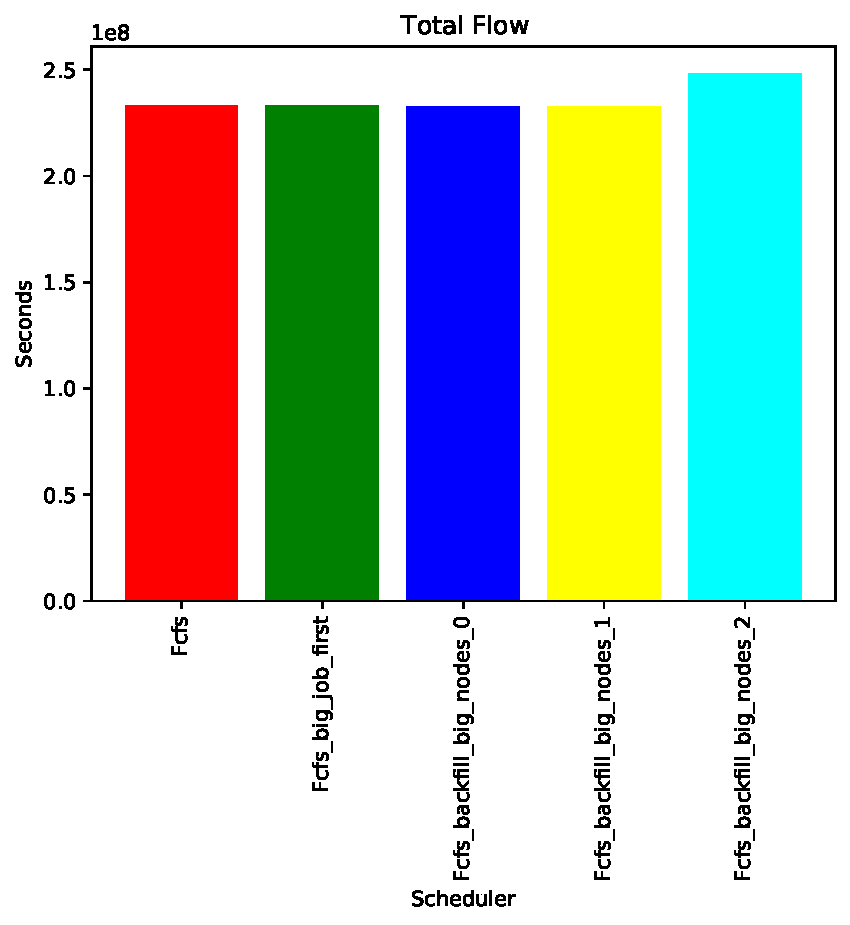
\includegraphics[width=1\linewidth]{MBSS/plot/Size_Constraint_2022-03-26->2022-03-26_classic_Total_flow_95_128_4_256_1_1024.pdf}\caption{Total flow}\end{subfigure}
	\begin{subfigure}[b]{0.4\linewidth}\centering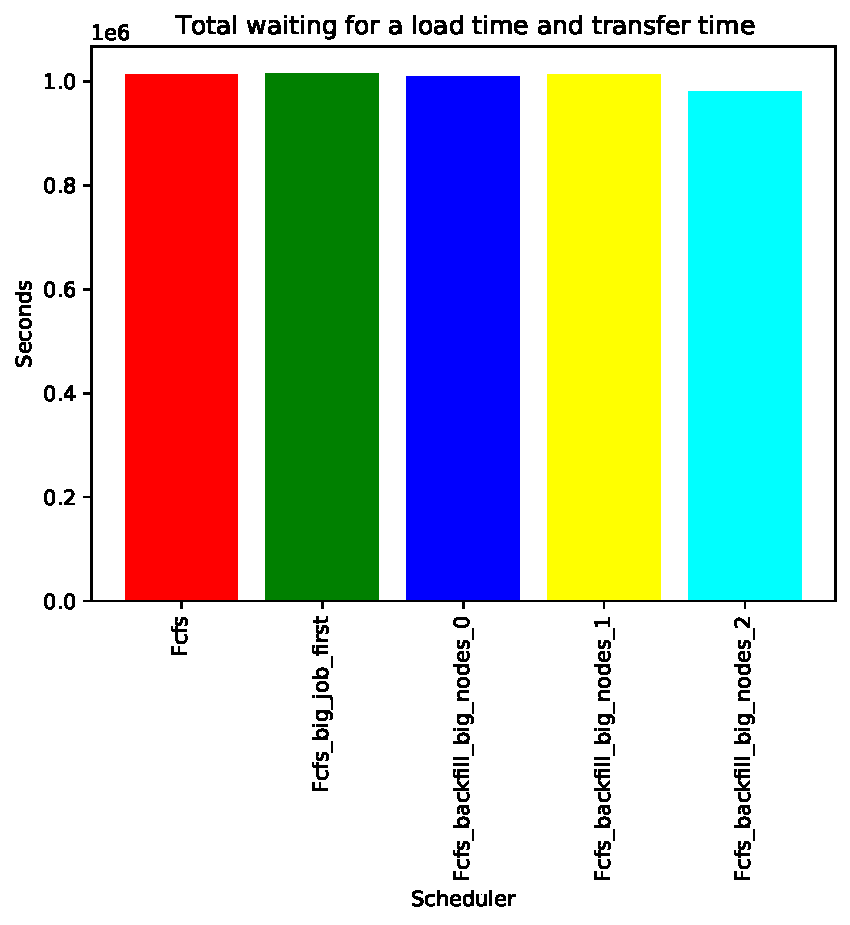
\includegraphics[width=1\linewidth]{MBSS/plot/Size_Constraint_2022-03-26->2022-03-26_classic_Total_waiting_for_a_load_time_and_transfer_time_95_128_4_256_1_1024.pdf}\caption{Waiting for a load and transfer time}\end{subfigure}\caption{Workload 2022-03-26\_classic - Performance on FCFS with constraint on files sizes - 1/4 cluster - May 30}\end{figure}
	
	\begin{figure}[H]\centering
	\begin{subfigure}[b]{0.4\linewidth}\centering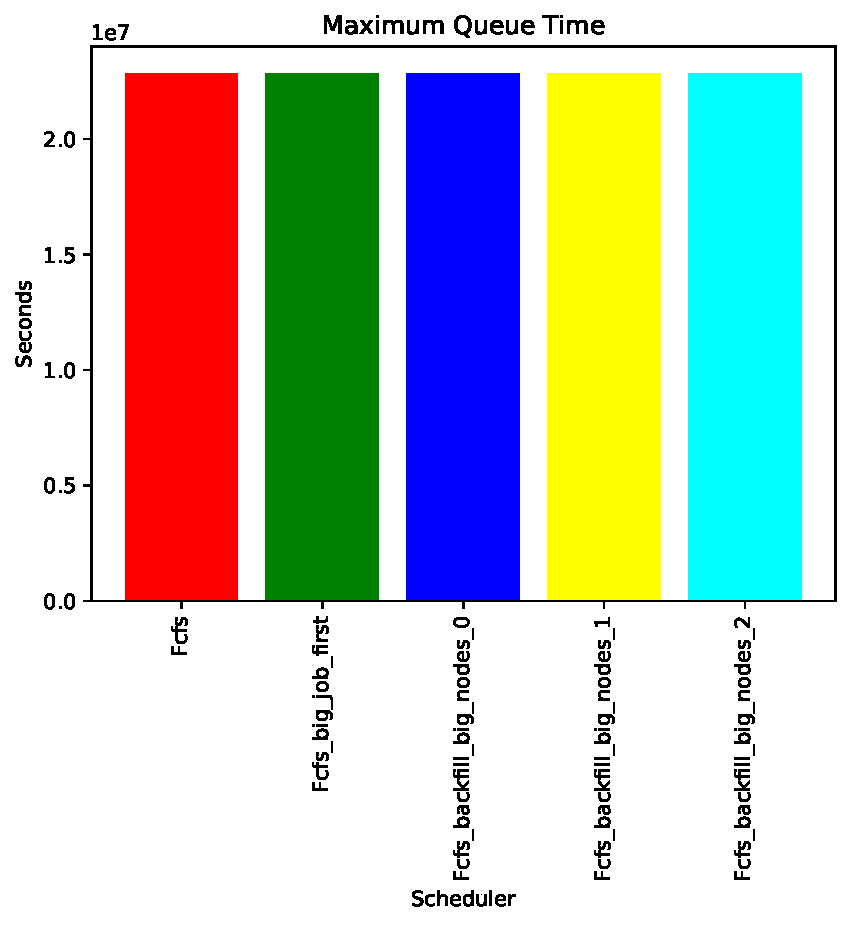
\includegraphics[width=1\linewidth]{MBSS/plot/Size_Constraint_2022-03-26->2022-03-26_Maximum_queue_time_95_128_4_256_1_1024.pdf}\caption{Maximum queue time}\end{subfigure}
	\begin{subfigure}[b]{0.4\linewidth}\centering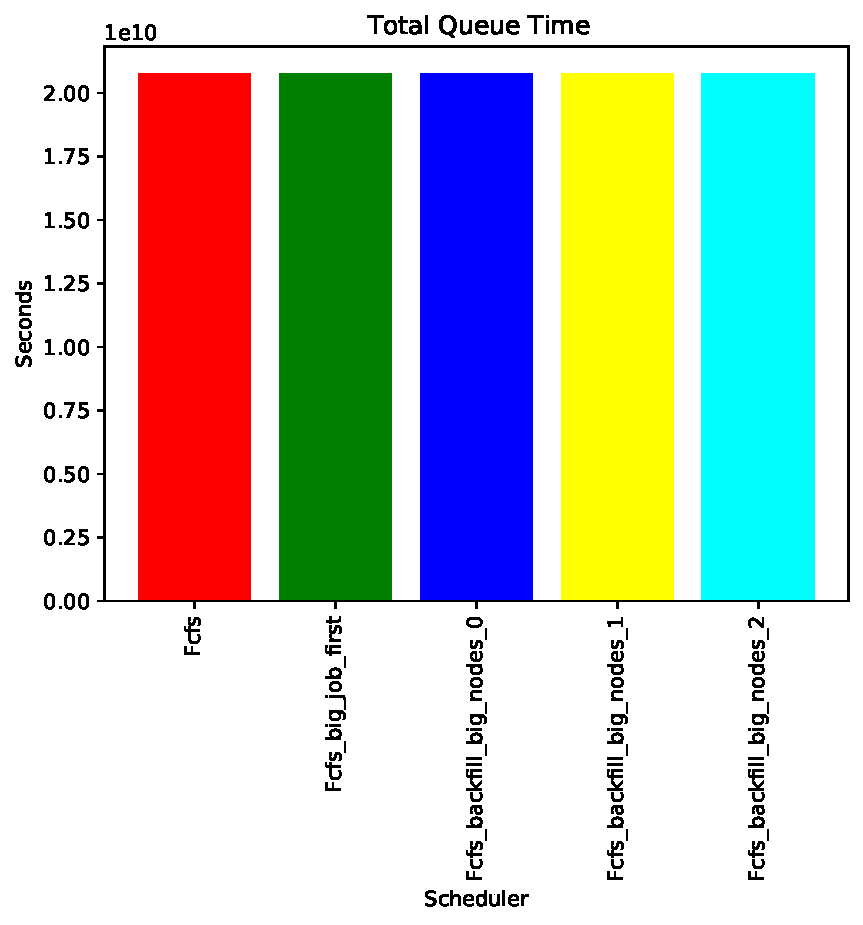
\includegraphics[width=1\linewidth]{MBSS/plot/Size_Constraint_2022-03-26->2022-03-26_Total_queue_time_95_128_4_256_1_1024.pdf}\caption{Total queue time}\end{subfigure}
	\begin{subfigure}[b]{0.4\linewidth}\centering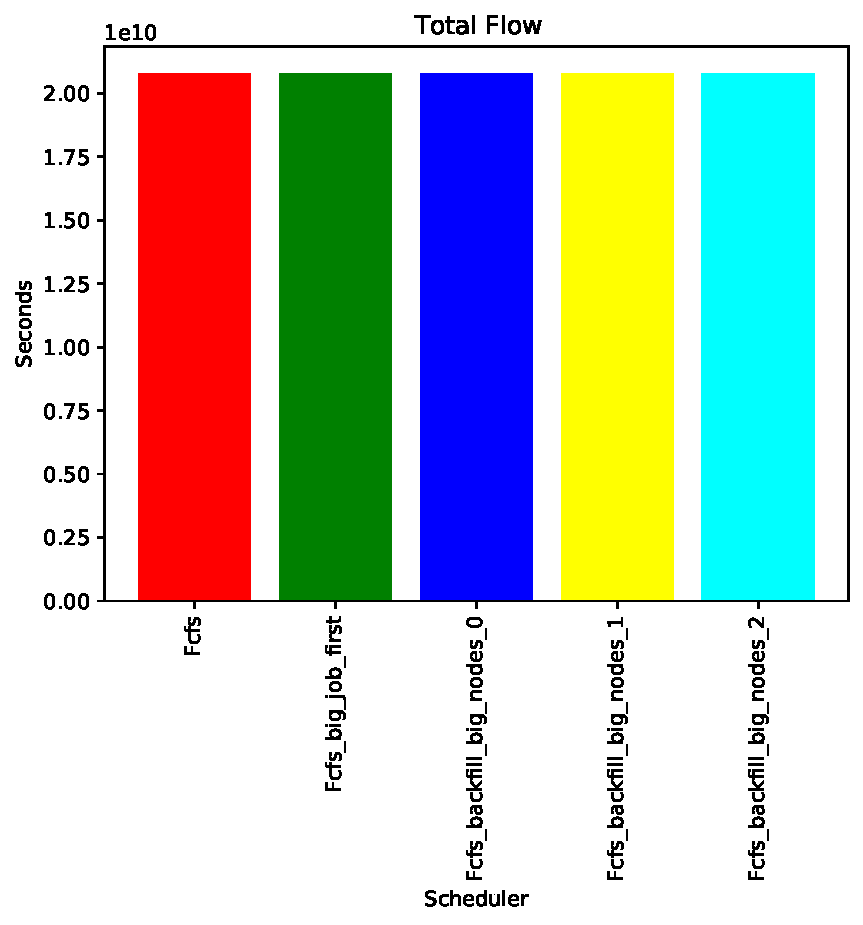
\includegraphics[width=1\linewidth]{MBSS/plot/Size_Constraint_2022-03-26->2022-03-26_Total_flow_95_128_4_256_1_1024.pdf}\caption{Total flow}\end{subfigure}
	\begin{subfigure}[b]{0.4\linewidth}\centering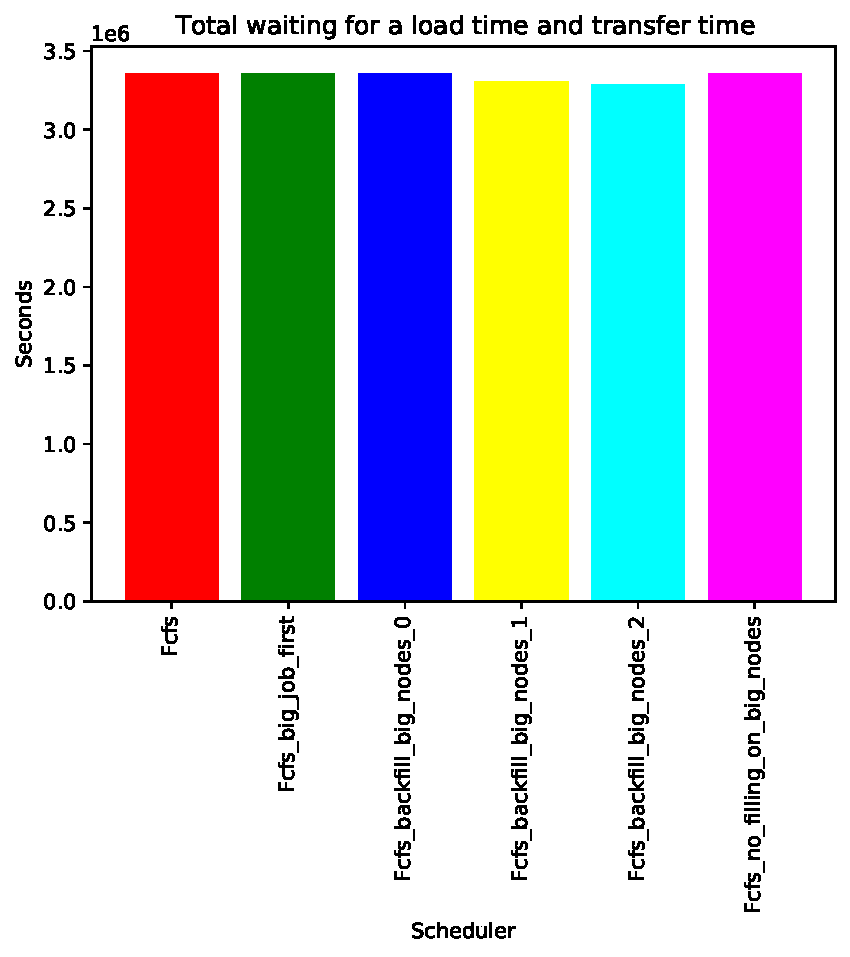
\includegraphics[width=1\linewidth]{MBSS/plot/Size_Constraint_2022-03-26->2022-03-26_Total_waiting_for_a_load_time_and_transfer_time_95_128_4_256_1_1024.pdf}\caption{Waiting for a load and transfer time}\end{subfigure}\caption{Workload 2022-03-26 - Performance on FCFS with constraint on files sizes - 1/4 cluster - May 30}\end{figure}


\section{Meeting 16/06/22}

\begin{figure}[H]\centering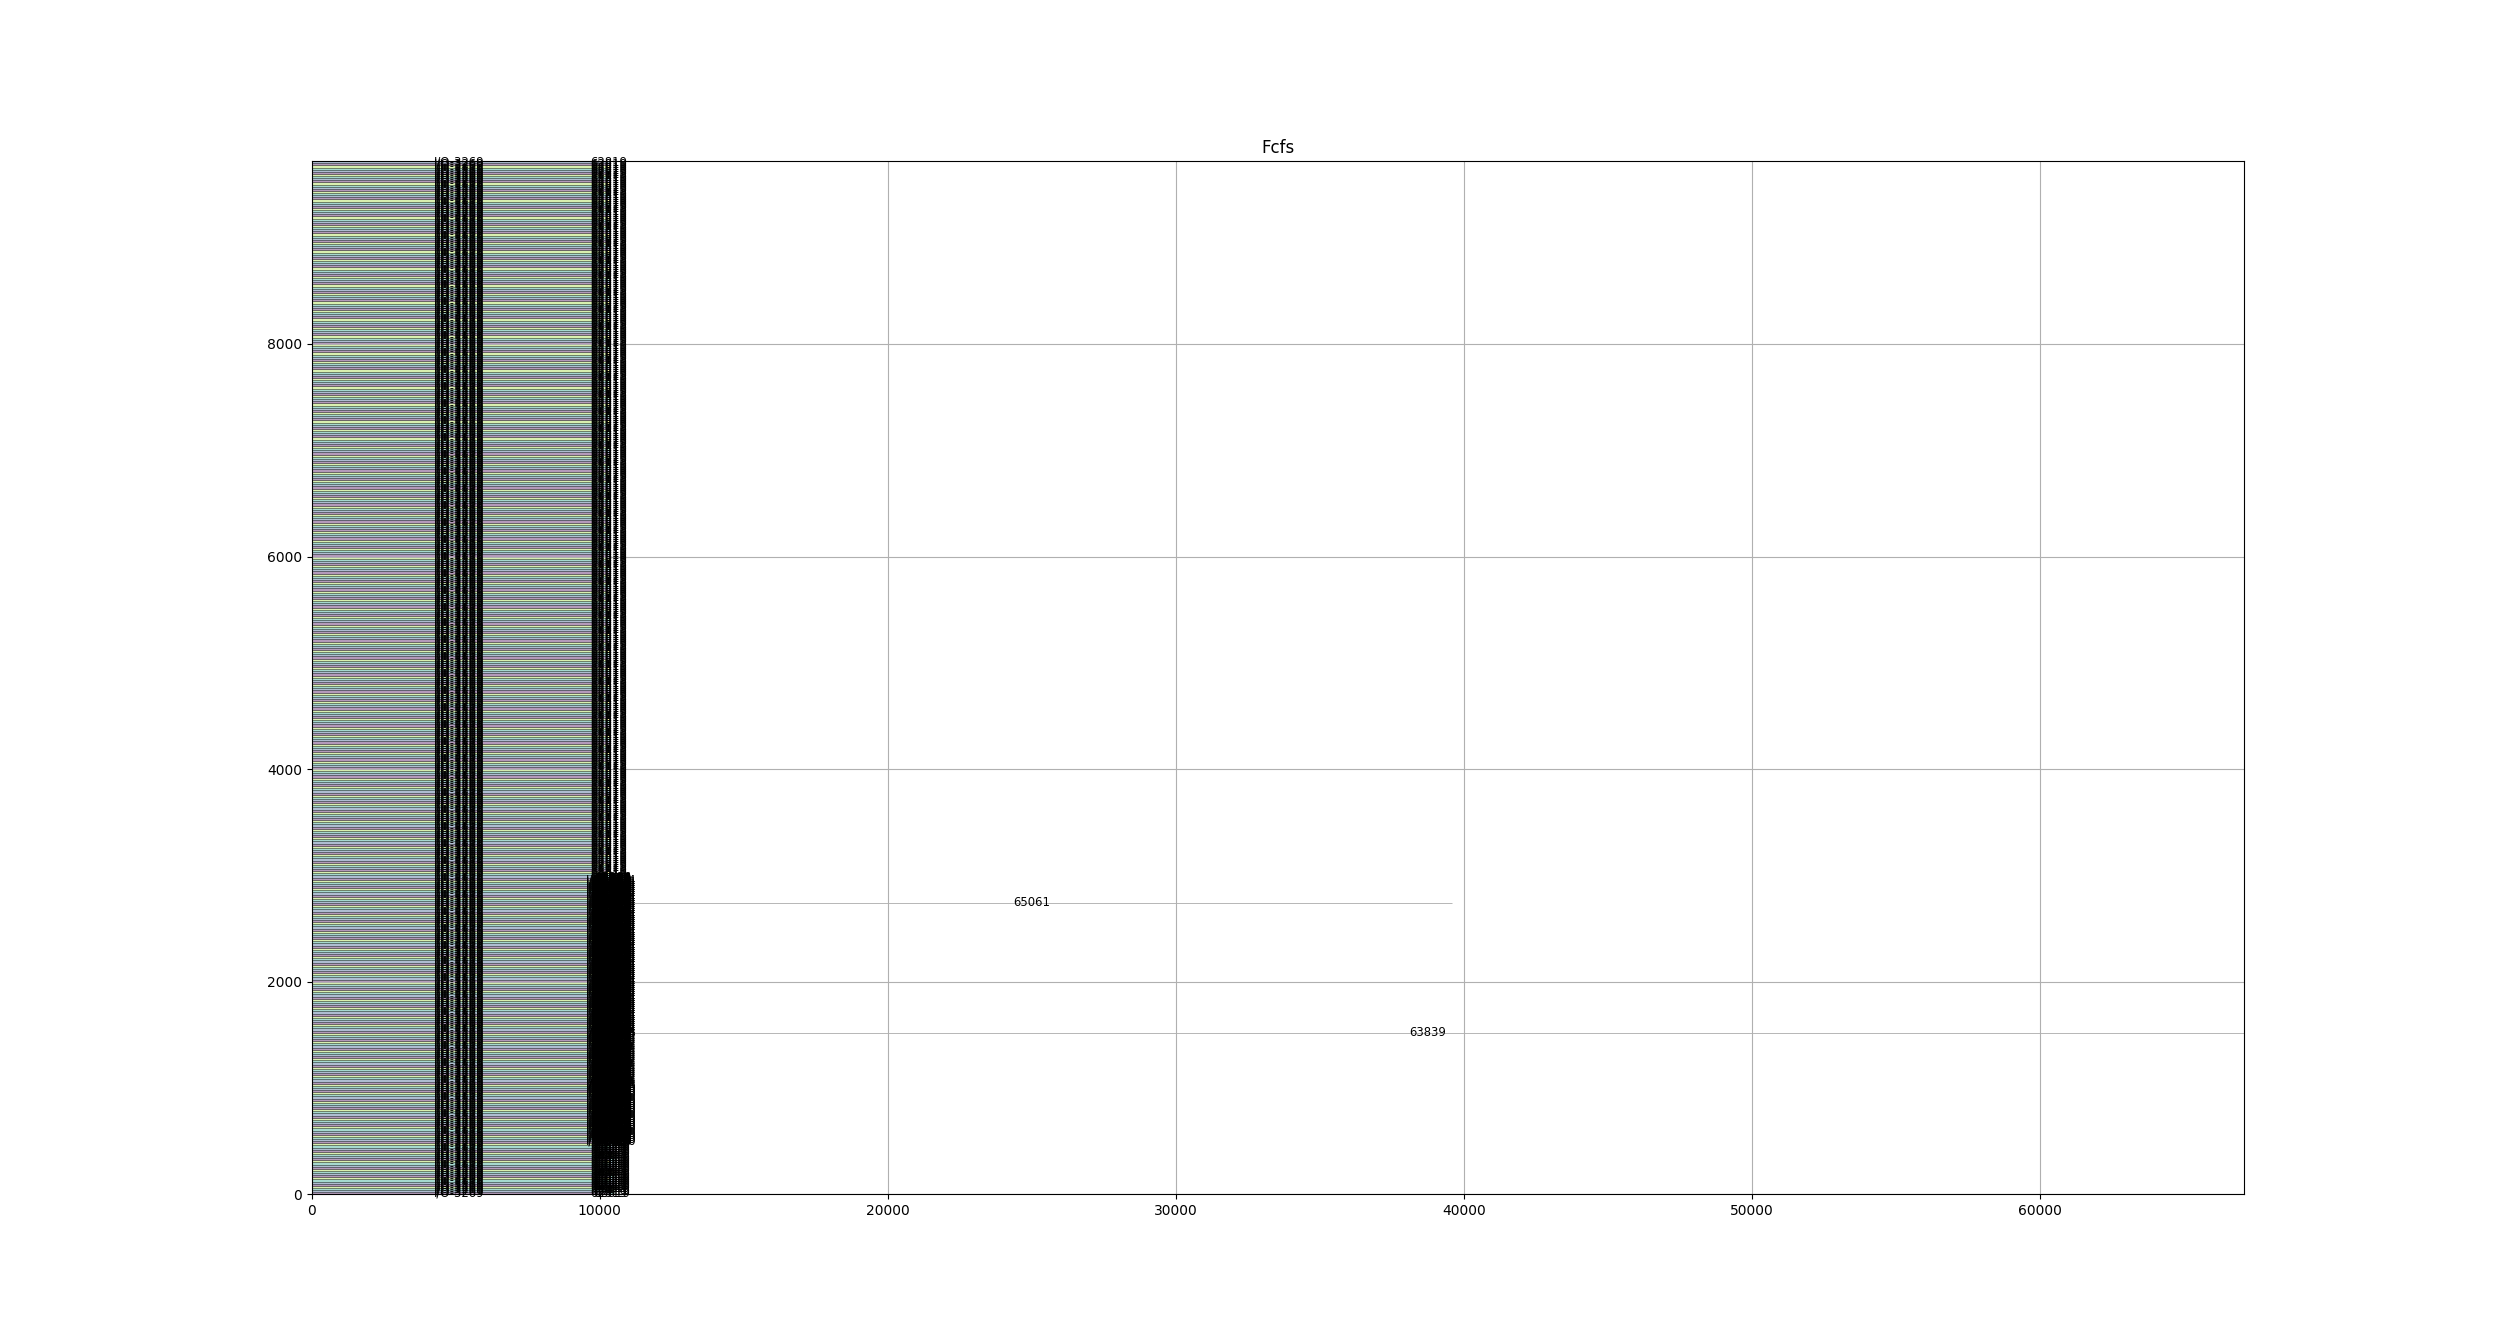
\includegraphics[width=1\linewidth]{MBSS/plot/Gantt_charts/Fcfs.png}\caption{FCFS}\end{figure}
\begin{figure}[H]\centering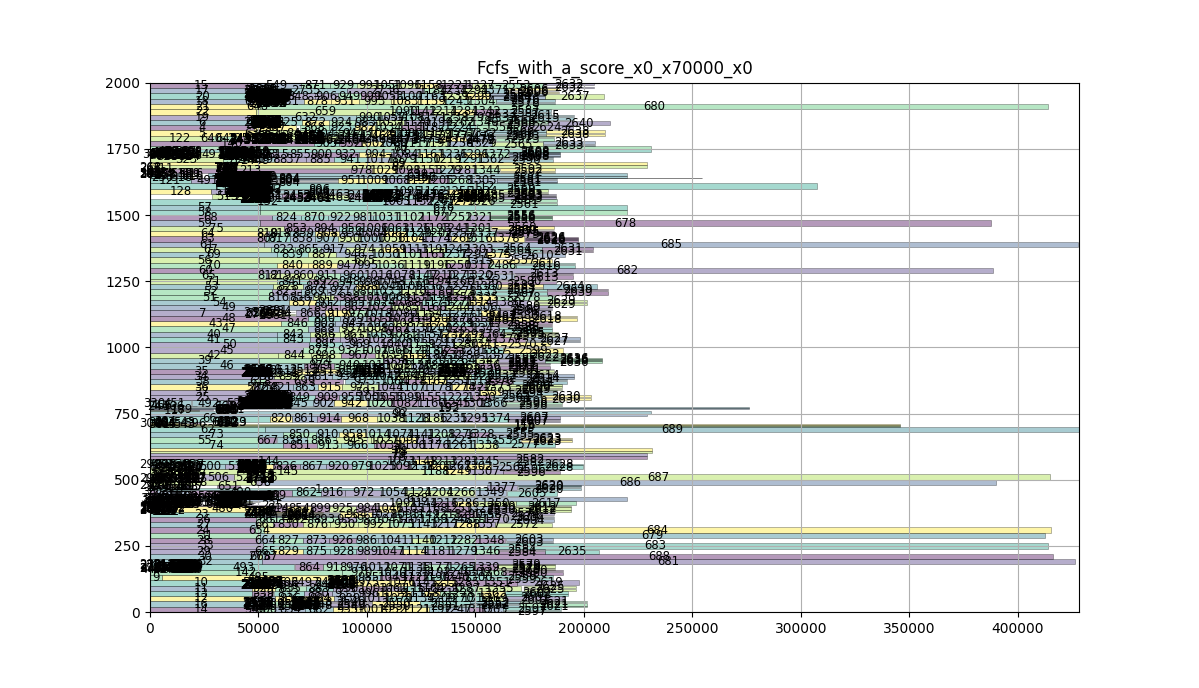
\includegraphics[width=1\linewidth]{MBSS/plot/Gantt_charts/Fcfs_with_a_score_x0_x70000_x0.png}\caption{FCFS with a score}\end{figure}
\begin{figure}[H]\centering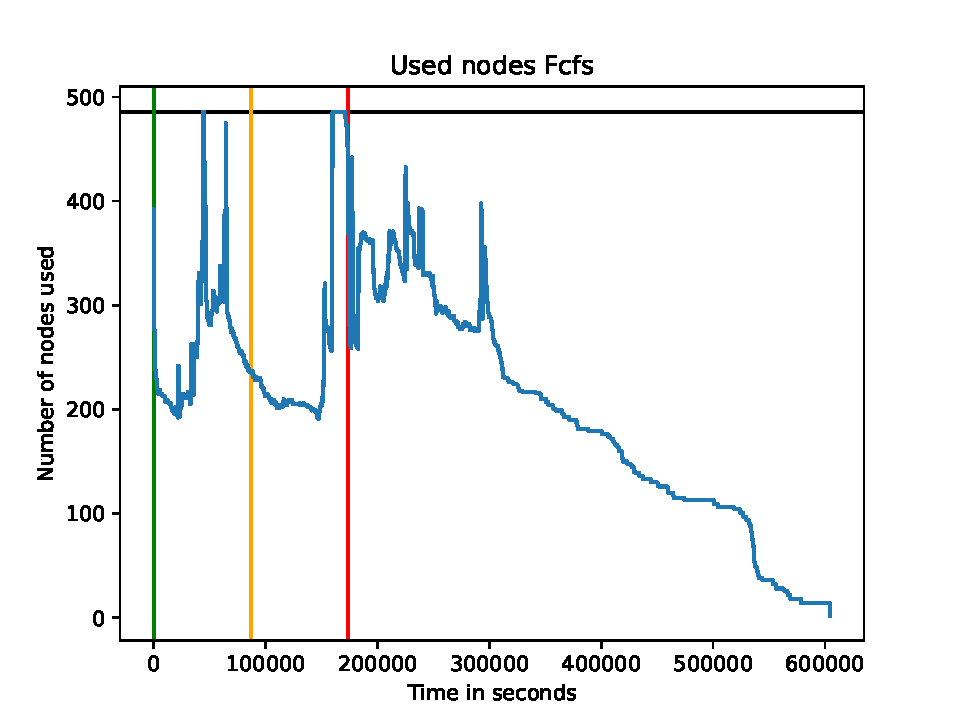
\includegraphics[width=1\linewidth]{MBSS/plot/plot_1.pdf}\caption{FCFS}\end{figure}
\begin{figure}[H]\centering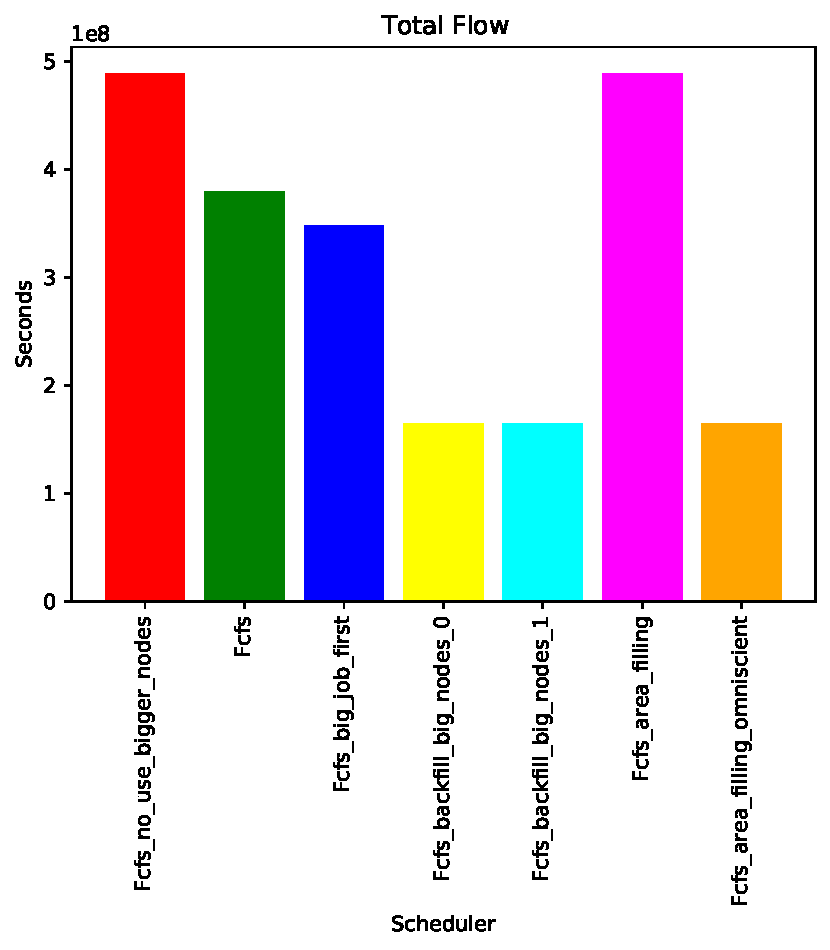
\includegraphics[width=1\linewidth]{MBSS/plot/Size_Constraint_2022-02-08->2022-02-08_very_reduced_Total_flow_95_128_4_256_1_1024.pdf}\caption{Size constraint}\end{figure}
For each size x I compute: Planned Area (3) : [ 0, 50, infinite ] \\
If I look into the past I get: Planned Area (3) : [ 0, 0, infinite ]
\begin{figure}[H]\centering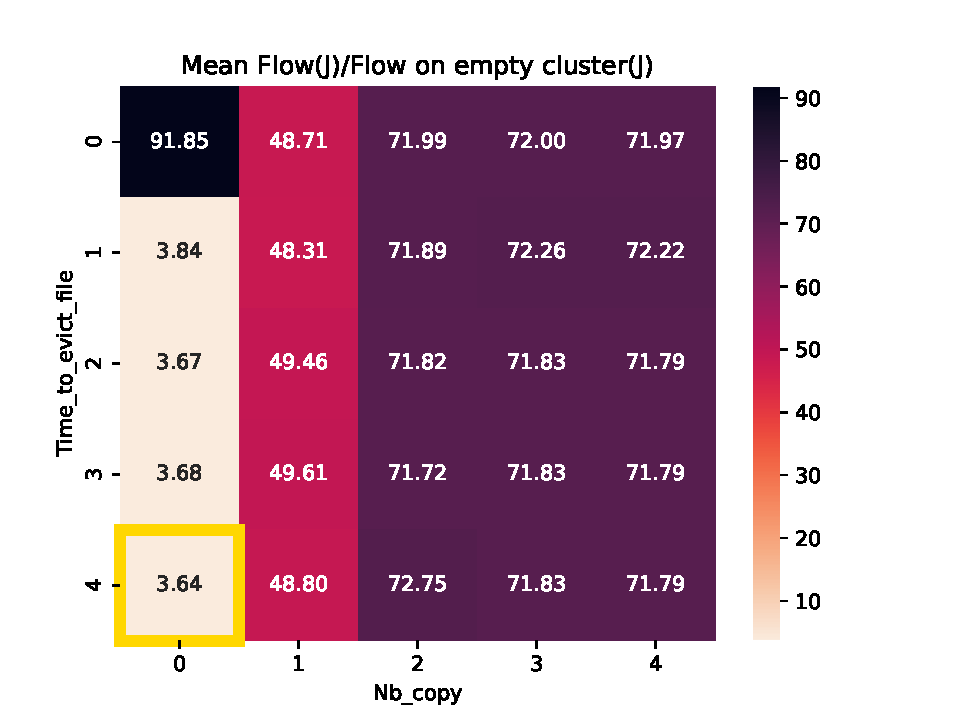
\includegraphics[width=1\linewidth]{MBSS/plot/FCFS_Score_Expe_V2/Heatmap_FCFS_Score_Time_to_evict_file_Nb_copy_2022-02-08->2022-02-08_very_reduced_95_128_4_256_1_1024.pdf}\caption{Heatmap FCFS with a score}\end{figure}
\begin{figure}[H]\centering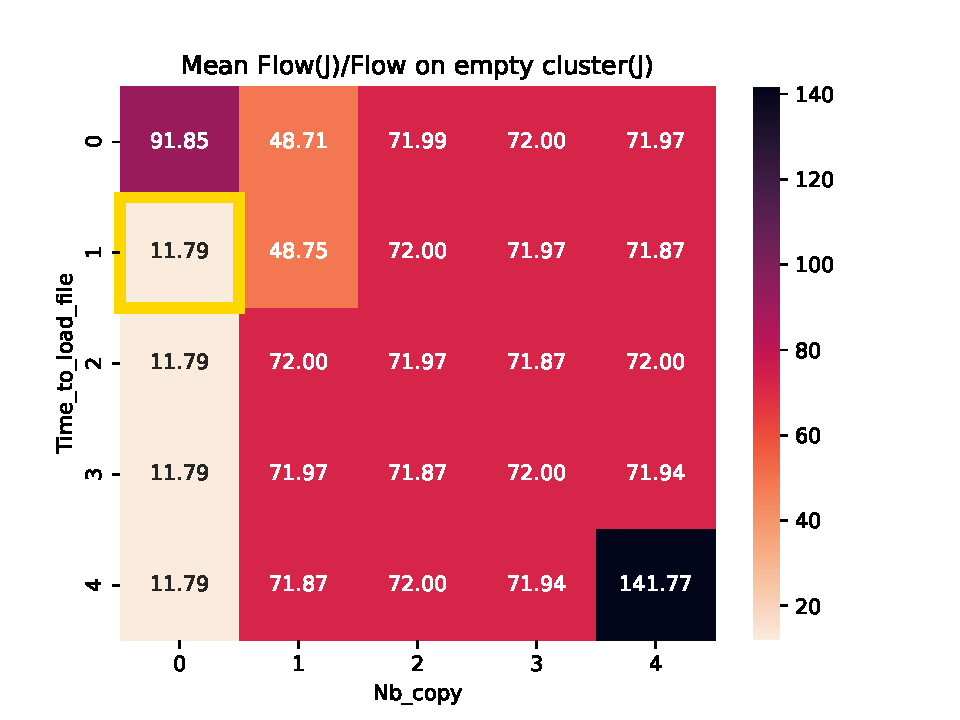
\includegraphics[width=1\linewidth]{MBSS/plot/FCFS_Score_Expe_V2/Heatmap_FCFS_Score_Time_to_load_file_Nb_copy_2022-02-08->2022-02-08_very_reduced_95_128_4_256_1_1024.pdf}\caption{}\end{figure}
\begin{figure}[H]\centering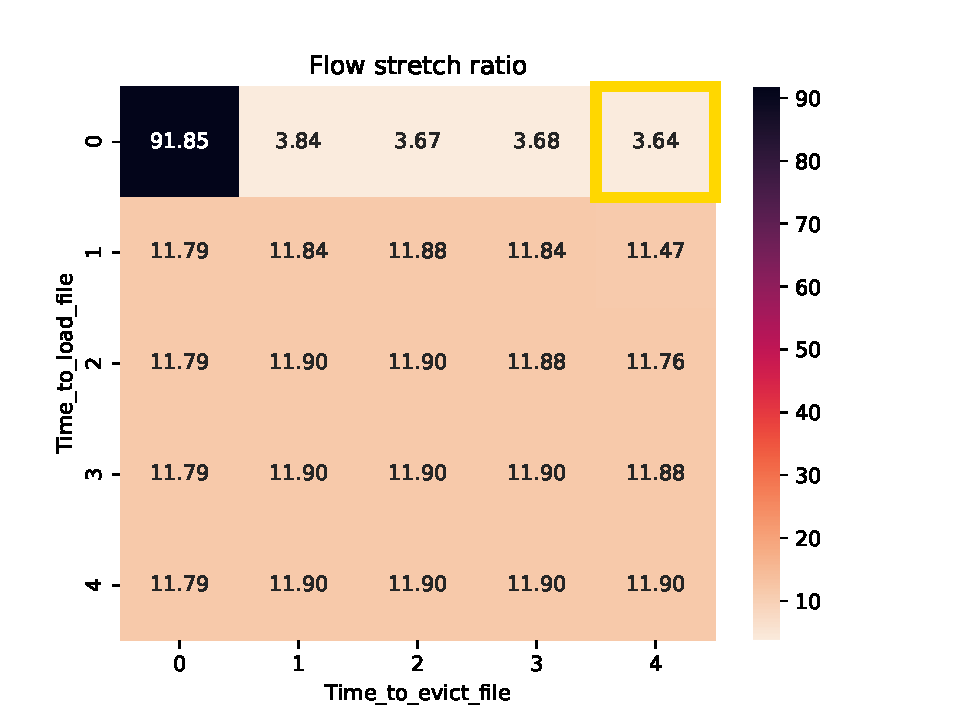
\includegraphics[width=1\linewidth]{MBSS/plot/FCFS_Score_Expe_V2/Heatmap_FCFS_Score_Time_to_load_file_Time_to_evict_file_2022-02-08->2022-02-08_very_reduced_95_128_4_256_1_1024.pdf}\caption{}\end{figure}
\begin{figure}[H]\centering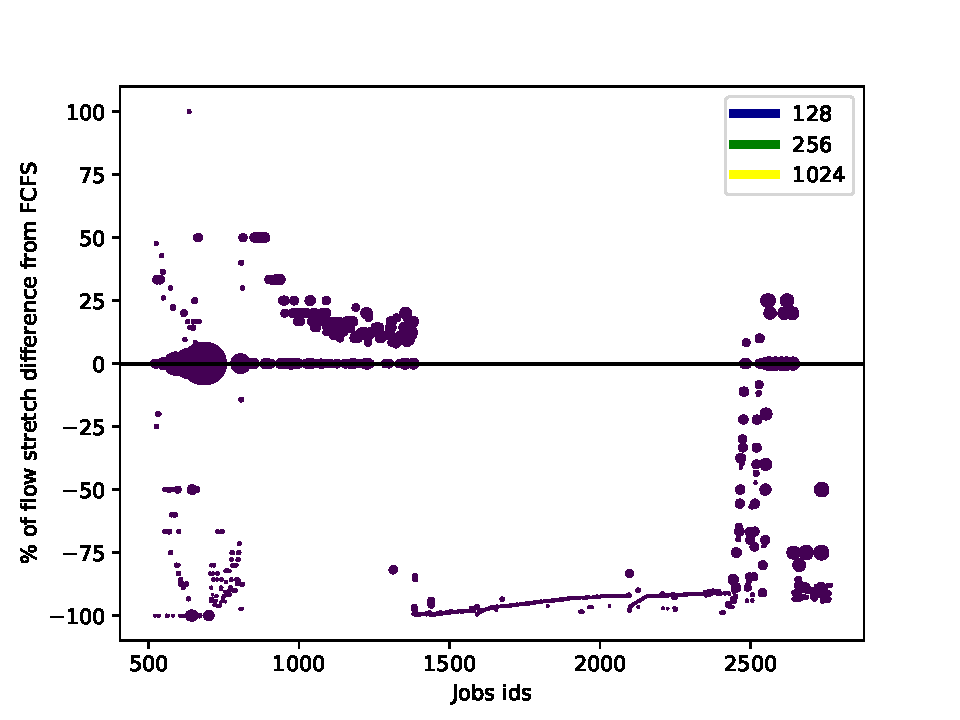
\includegraphics[width=1\linewidth]{MBSS/plot/FCFRSvsfcfsscore.pdf}\caption{}\end{figure}

\section{Meeting 23/06/22}

\begin{figure}[H]\centering
\begin{subfigure}[b]{0.4\linewidth}\centering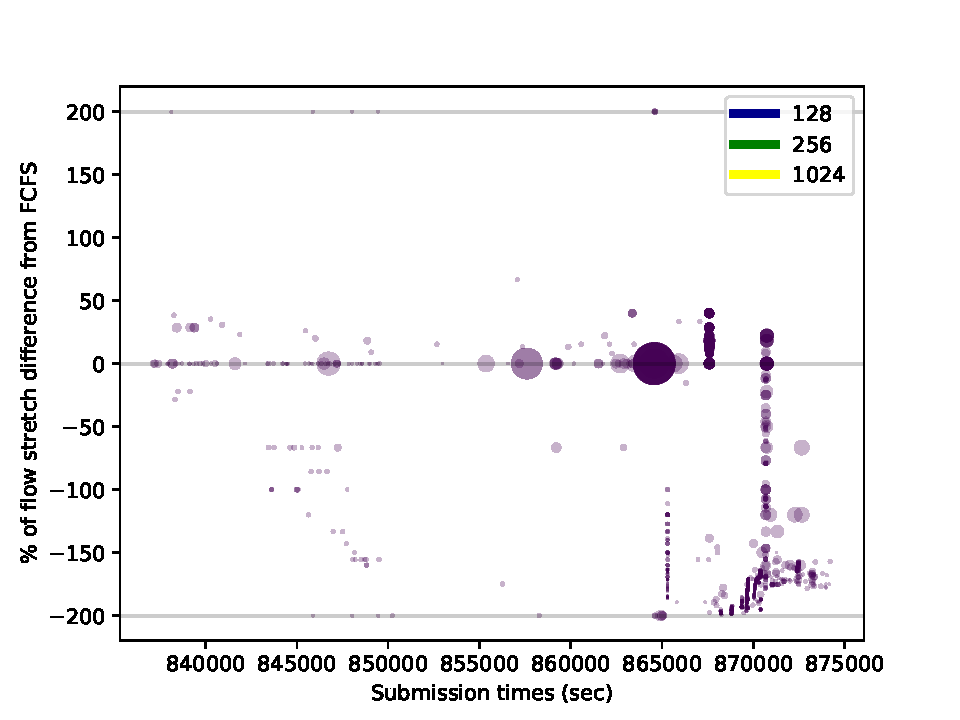
\includegraphics[width=1\linewidth]{MBSS/plot/Stretch_times_Fcfs_Fcfs_with_a_score_x0_x70000_x0_2022-02-08->2022-02-08_reduced_95_128_4_256_1_1024.pdf}\caption{Stretch}\end{subfigure}
\begin{subfigure}[b]{0.4\linewidth}\centering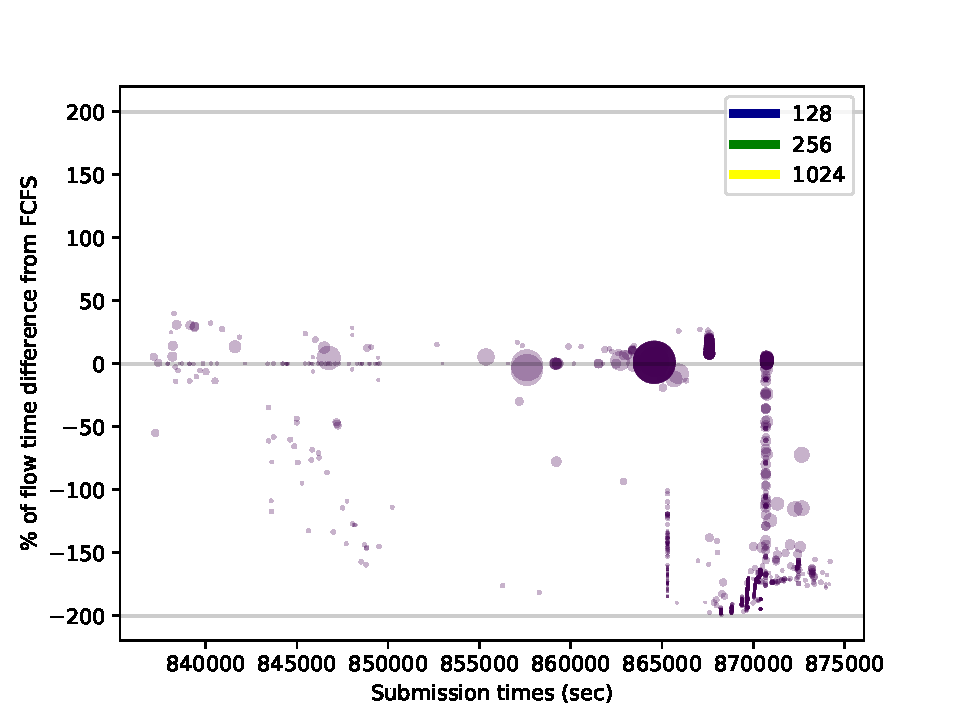
\includegraphics[width=1\linewidth]{MBSS/plot/Flow_times_Fcfs_Fcfs_with_a_score_x0_x70000_x0_2022-02-08->2022-02-08_reduced_95_128_4_256_1_1024.pdf}\caption{Flow}\end{subfigure}
\begin{subfigure}[b]{0.4\linewidth}\centering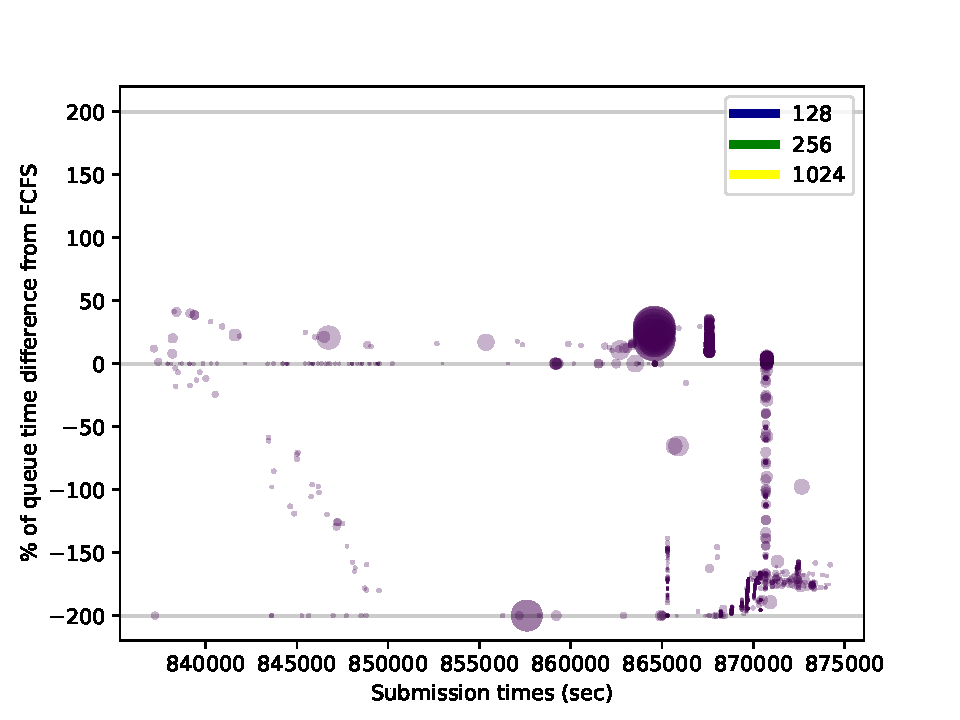
\includegraphics[width=1\linewidth]{MBSS/plot/Queue_times_Fcfs_Fcfs_with_a_score_x0_x70000_x0_2022-02-08->2022-02-08_reduced_95_128_4_256_1_1024.pdf}\caption{Queue}\end{subfigure}\caption{FCFS VS FCFS with a score x0 x7000 x0 - June 17 - New plots for percentage difference ($percentage~difference = 100 * |a - b| / ((a + b) / 2)$) with 200\% if one value is at 0. FCFS VS FCFS with a score.}\end{figure}

\begin{figure}[H]\centering
\begin{subfigure}[b]{0.4\linewidth}\centering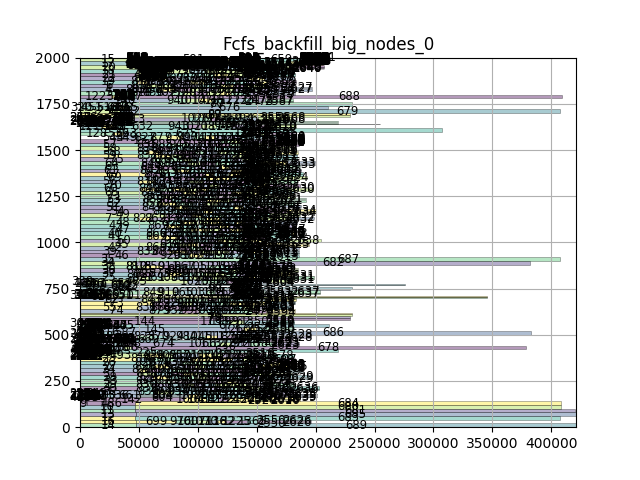
\includegraphics[width=1\linewidth]{MBSS/plot/Gantt_charts/Fcfs_backfill_big_nodes_0.png}\caption{FCFS backfill big nodes}\end{subfigure}
\begin{subfigure}[b]{0.4\linewidth}\centering\includegraphics[width=1\linewidth]{MBSS/plot/Gantt_charts/Fcfs_no_use_bigger_nodes.png}\caption{FCFS no use bigger nodes}\end{subfigure}
\begin{subfigure}[b]{0.4\linewidth}\centering\includegraphics[width=1\linewidth]{MBSS/plot/Flow_times_Fcfs_no_use_bigger_nodes_Fcfs_backfill_big_nodes_0_2022-02-08->2022-02-08_reduced_95_128_4_256_1_1024.pdf}\caption{Flow}\end{subfigure}
\caption{Size constraint - June 17 - Trace size constraint to understand big total flow difference (192903568 VS 139565444).}\end{figure}

\section{Meeting ??/??/22}

\subsection{Finding parameters for FCFS with a score}

No constraint on node sizes.

\begin{figure}[H]\centering
\begin{subfigure}[b]{0.4\linewidth}\centering\includegraphics[width=1\linewidth]{MBSS/plot/Heatmap_Stretch_FCFS_Score_Time_to_load_file_Time_to_evict_file_2022-01-24->2022-01-24_450_128_32_256_4_1024.pdf}\caption{Mean Flow Stretch}\end{subfigure}
\begin{subfigure}[b]{0.4\linewidth}\centering\includegraphics[width=1\linewidth]{MBSS/plot/Heatmap_Max_Stretch_FCFS_Score_Time_to_load_file_Time_to_evict_file_2022-01-24->2022-01-24_450_128_32_256_4_1024.pdf}\caption{Max Flow Stretch}\end{subfigure}
\begin{subfigure}[b]{0.4\linewidth}\centering\includegraphics[width=1\linewidth]{MBSS/plot/Heatmap_Stretch_with_a_minimum_FCFS_Score_Time_to_load_file_Time_to_evict_file_2022-01-24->2022-01-24_450_128_32_256_4_1024.pdf}\caption{Mean Bounded Flow Stretch $(T/max(T_{opti}, 5min))$}\end{subfigure}
\begin{subfigure}[b]{0.4\linewidth}\centering\includegraphics[width=1\linewidth]{MBSS/plot/Heatmap_Max_Stretch_with_a_minimum_FCFS_Score_Time_to_load_file_Time_to_evict_file_2022-01-24->2022-01-24_450_128_32_256_4_1024.pdf}\caption{Max Bounded Flow Stretch}\end{subfigure}
\begin{subfigure}[b]{0.4\linewidth}\centering\includegraphics[width=1\linewidth]{MBSS/plot/Heatmap_Total_Flow_FCFS_Score_Time_to_load_file_Time_to_evict_file_2022-01-24->2022-01-24_450_128_32_256_4_1024.pdf}\caption{Total Flow}\end{subfigure}
\begin{subfigure}[b]{0.4\linewidth}\centering\includegraphics[width=1\linewidth]{MBSS/plot/Heatmap_Max_Flow_FCFS_Score_Time_to_load_file_Time_to_evict_file_2022-01-24->2022-01-24_450_128_32_256_4_1024.pdf}\caption{Max Flow}\end{subfigure}
\caption{Time to load a file X Time to evict files - June 30}\end{figure}

\begin{figure}[H]\centering
\begin{subfigure}[b]{0.4\linewidth}\centering\includegraphics[width=1\linewidth]{MBSS/plot/Heatmap_Stretch_FCFS_Score_Time_to_load_file_Nb_copy_2022-01-24->2022-01-24_450_128_32_256_4_1024.pdf}\caption{Mean Flow Stretch}\end{subfigure}
\begin{subfigure}[b]{0.4\linewidth}\centering\includegraphics[width=1\linewidth]{MBSS/plot/Heatmap_Max_Stretch_FCFS_Score_Time_to_load_file_Nb_copy_2022-01-24->2022-01-24_450_128_32_256_4_1024.pdf}\caption{Max Flow Stretch}\end{subfigure}
\begin{subfigure}[b]{0.4\linewidth}\centering\includegraphics[width=1\linewidth]{MBSS/plot/Heatmap_Stretch_with_a_minimum_FCFS_Score_Time_to_load_file_Nb_copy_2022-01-24->2022-01-24_450_128_32_256_4_1024.pdf}\caption{Mean Bounded Flow Stretch $(T/max(T_{opti}, 5min))$}\end{subfigure}
\begin{subfigure}[b]{0.4\linewidth}\centering\includegraphics[width=1\linewidth]{MBSS/plot/Heatmap_Max_Stretch_with_a_minimum_FCFS_Score_Time_to_load_file_Nb_copy_2022-01-24->2022-01-24_450_128_32_256_4_1024.pdf}\caption{Max Bounded Flow Stretch}\end{subfigure}
\begin{subfigure}[b]{0.4\linewidth}\centering\includegraphics[width=1\linewidth]{MBSS/plot/Heatmap_Total_Flow_FCFS_Score_Time_to_load_file_Nb_copy_2022-01-24->2022-01-24_450_128_32_256_4_1024.pdf}\caption{Total Flow}\end{subfigure}
\begin{subfigure}[b]{0.4\linewidth}\centering\includegraphics[width=1\linewidth]{MBSS/plot/Heatmap_Max_Flow_FCFS_Score_Time_to_load_file_Nb_copy_2022-01-24->2022-01-24_450_128_32_256_4_1024.pdf}\caption{Max Flow}\end{subfigure}
\caption{Time to load a file X Number of copy of a file - July 1}\end{figure}

\begin{figure}[H]\centering
\begin{subfigure}[b]{0.4\linewidth}\centering\includegraphics[width=1\linewidth]{MBSS/plot/Heatmap_Stretch_FCFS_Score_Time_to_evict_file_Nb_copy_2022-01-24->2022-01-24_450_128_32_256_4_1024.pdf}\caption{Mean Flow Stretch}\end{subfigure}
\begin{subfigure}[b]{0.4\linewidth}\centering\includegraphics[width=1\linewidth]{MBSS/plot/Heatmap_Max_Stretch_FCFS_Score_Time_to_evict_file_Nb_copy_2022-01-24->2022-01-24_450_128_32_256_4_1024.pdf}\caption{Max Flow Stretch}\end{subfigure}
\begin{subfigure}[b]{0.4\linewidth}\centering\includegraphics[width=1\linewidth]{MBSS/plot/Heatmap_Stretch_with_a_minimum_FCFS_Score_Time_to_evict_file_Nb_copy_2022-01-24->2022-01-24_450_128_32_256_4_1024.pdf}\caption{Mean Bounded Flow Stretch $(T/max(T_{opti}, 5min))$}\end{subfigure}
\begin{subfigure}[b]{0.4\linewidth}\centering\includegraphics[width=1\linewidth]{MBSS/plot/Heatmap_Max_Stretch_with_a_minimum_FCFS_Score_Time_to_evict_file_Nb_copy_2022-01-24->2022-01-24_450_128_32_256_4_1024.pdf}\caption{Max Bounded Flow Stretch}\end{subfigure}
\begin{subfigure}[b]{0.4\linewidth}\centering\includegraphics[width=1\linewidth]{MBSS/plot/Heatmap_Total_Flow_FCFS_Score_Time_to_evict_file_Nb_copy_2022-01-24->2022-01-24_450_128_32_256_4_1024.pdf}\caption{Total Flow}\end{subfigure}
\begin{subfigure}[b]{0.4\linewidth}\centering\includegraphics[width=1\linewidth]{MBSS/plot/Heatmap_Max_Flow_FCFS_Score_Time_to_evict_file_Nb_copy_2022-01-24->2022-01-24_450_128_32_256_4_1024.pdf}\caption{Max Flow}\end{subfigure}
\caption{Time to evict a file X Number of copy of a file - July 8}\end{figure}

\begin{figure}[H]\centering
\begin{subfigure}[b]{0.4\linewidth}\centering\includegraphics[width=1\linewidth]{MBSS/plot/FCFS_Score_2022-01-24->2022-01-24_Total_waiting_for_a_load_time_and_transfer_time_450_128_32_256_4_1024.pdf}\caption{Transfer and waiting for a load time}\label{1}\end{subfigure}
\begin{subfigure}[b]{0.4\linewidth}\centering\includegraphics[width=1\linewidth]{MBSS/plot/FCFS_Score_2022-01-24->2022-01-24_Makespan_450_128_32_256_4_1024.pdf}\caption{Makespan}\label{2}\end{subfigure}
\begin{subfigure}[b]{0.4\linewidth}\centering\includegraphics[width=1\linewidth]{MBSS/plot/FCFS_Score_2022-01-24->2022-01-24_Core_time_used_450_128_32_256_4_1024.pdf}\caption{Core time used}\end{subfigure}
\begin{subfigure}[b]{0.4\linewidth}\centering\includegraphics[width=1\linewidth]{MBSS/plot/FCFS_Score_2022-01-24->2022-01-24_Maximum_queue_time_450_128_32_256_4_1024.pdf}\caption{Max queue time}\label{0}\end{subfigure}
\caption{Comparing multiplier for FCFS with a score - July 8}\end{figure}

\paragraph {Conclusion on finding parameters for FCFS with a score}
\begin{itemize}
	\item The nb of copy parameters gives us worse performances. As we can see on figure \ref{1} and \ref{2}, it reduces
	the amount of data transfers because it does not want to create ne copy but at the expense of the makespan. Which means that 
	you have very bad load balance.
	\item The best parameters for time to load a file and time to evict a file are 500 500 for the mean bounded and un-bounded stretch as well as for the max bounded stretch and total flow. For the max flow, we can see that it's better to put at 0 the time to load file. In this situation you are not constrained when choosing a node by the common data and you can thus have a better load balance and thus avoid waiting for a good node in term of locality which give fewer risk of having a very long flow on a job.
\end{itemize}

\subsection{Trying EASY-backfilling}

No constraint on node sizes.

\begin{figure}[H]\centering
\begin{subfigure}[b]{0.4\linewidth}\centering\includegraphics[width=1\linewidth]{MBSS/plot/Backfill_2022-01-24->2022-01-24_Total_waiting_for_a_load_time_and_transfer_time_450_128_32_256_4_1024.pdf}\caption{Transfer and waiting for a load time}\label{3}\end{subfigure}
\begin{subfigure}[b]{0.4\linewidth}\centering\includegraphics[width=1\linewidth]{MBSS/plot/Backfill_2022-01-24->2022-01-24_Mean_Stretch_With_a_Minimum_450_128_32_256_4_1024.pdf}\caption{Mean bounded stretch}\label{4}\end{subfigure}
\begin{subfigure}[b]{0.4\linewidth}\centering\includegraphics[width=1\linewidth]{MBSS/plot/Backfill_2022-01-24->2022-01-24_Maximum_queue_time_450_128_32_256_4_1024.pdf}\caption{Maximum queue time}\label{5}\end{subfigure}
\begin{subfigure}[b]{0.4\linewidth}\centering\includegraphics[width=1\linewidth]{MBSS/plot/Backfill_2022-01-24->2022-01-24_Total_flow_450_128_32_256_4_1024.pdf}\caption{Total flow}\label{6}\end{subfigure}
\caption{Comparing algorithms with EASY-backfill - Sometime in July}\end{figure}

\paragraph {Conclusion on trying EASY-backfilling}
\begin{itemize}
	\item From figure \ref{4} and \ref{6}, we can see that fcfs benefit from EASY-backfilling.
	\item From figure \ref{4} and \ref{6}, we can see that fcfs with a score does not benefit from EASY-backfilling. It can be explained by the greater amount of transfers that we can see on figure \ref{3}. My conclusion on this was first to 
	try with conservative backfilling. But with this you still loose data locality because any backfilling will replace the node's memory. So my goal will simply be here to try without backfilling at all and consider that the gain on transfer time is too important to be put as a secondary objective.
	\item From figure \ref{5}, we can see that fcfs with a score suffer from a significantly higher max queue time that the other algorithms. We can already see it on figure \ref{0}. Indeed, waiting for a better node for locality will increase waiting time for a few jobs. Now the question is, does this happen on a large amount of jobs ? Maybe I should plot the number of jobs where the queue time is superior to 25000 for example ? If it's only a few jobs we can consider that it's not important ?
\end{itemize}

\end{document}
